\documentclass[a4paper]{book}
\usepackage{makeidx}
\usepackage{graphicx}
\usepackage{multicol}
\usepackage{float}
\usepackage{listings}
\usepackage{color}
\usepackage{ifthen}
\usepackage[table]{xcolor}
\usepackage{textcomp}
\usepackage{alltt}
\usepackage{ifpdf}
\ifpdf
\usepackage[pdftex,
            pagebackref=true,
            colorlinks=true,
            linkcolor=blue,
            unicode
           ]{hyperref}
\else
\usepackage[ps2pdf,
            pagebackref=true,
            colorlinks=true,
            linkcolor=blue,
            unicode
           ]{hyperref}
\usepackage{pspicture}
\fi
\usepackage[utf8]{inputenc}
\usepackage{mathptmx}
\usepackage[scaled=.90]{helvet}
\usepackage{courier}
\usepackage{doxygen}
\lstset{language=C++,inputencoding=utf8,basicstyle=\footnotesize,breaklines=true,breakatwhitespace=true,tabsize=8,numbers=left }
\makeindex
\setcounter{tocdepth}{3}
\renewcommand{\footrulewidth}{0.4pt}
\begin{document}
\hypersetup{pageanchor=false}
\begin{titlepage}
\vspace*{7cm}
\begin{center}
{\Large Shift Stepper \\[1ex]\large v0.01a }\\
\vspace*{1cm}
{\large Generated by Doxygen 1.7.2}\\
\vspace*{0.5cm}
{\small Thu Dec 9 2010 20:57:05}\\
\end{center}
\end{titlepage}
\clearemptydoublepage
\pagenumbering{roman}
\tableofcontents
\clearemptydoublepage
\pagenumbering{arabic}
\hypersetup{pageanchor=true}
\chapter{Class Index}
\section{Class Hierarchy}
This inheritance list is sorted roughly, but not completely, alphabetically:\begin{DoxyCompactList}
\item \contentsline{section}{shiftChain}{\pageref{classshift_chain}}{}
\item \contentsline{section}{shiftDevice}{\pageref{classshift_device}}{}
\begin{DoxyCompactList}
\item \contentsline{section}{shiftStepMotor}{\pageref{classshift_step_motor}}{}
\item \contentsline{section}{shiftSwitchBlock}{\pageref{classshift_switch_block}}{}
\end{DoxyCompactList}
\item \contentsline{section}{shiftSix}{\pageref{classshift_six}}{}
\item \contentsline{section}{shiftSixteen}{\pageref{classshift_sixteen}}{}
\end{DoxyCompactList}

\chapter{Class Index}
\section{Class List}
Here are the classes, structs, unions and interfaces with brief descriptions:\begin{DoxyCompactList}
\item\contentsline{section}{\hyperlink{classshift_chain}{shiftChain} (Class to represent a daisy chain of boards )}{\pageref{classshift_chain}}{}
\item\contentsline{section}{\hyperlink{classshift_device}{shiftDevice} (Abstract base class for creating devices such as motors that attach to a board )}{\pageref{classshift_device}}{}
\item\contentsline{section}{\hyperlink{classshift_six}{shiftSix} (Implementation of shiftBoard for a six channel high current Arduino shield )}{\pageref{classshift_six}}{}
\item\contentsline{section}{\hyperlink{classshift_sixteen}{shiftSixteen} (Implementation of shiftBoard for a sixteen channel high current Arduino shield )}{\pageref{classshift_sixteen}}{}
\item\contentsline{section}{\hyperlink{classshift_step_motor}{shiftStepMotor} (Implementation of a 4-\/phase unipolar stepper motor device )}{\pageref{classshift_step_motor}}{}
\item\contentsline{section}{\hyperlink{classshift_switch_block}{shiftSwitchBlock} (A block of plain switches )}{\pageref{classshift_switch_block}}{}
\end{DoxyCompactList}

\chapter{File Index}
\section{File List}
Here is a list of all files with brief descriptions:\begin{DoxyCompactList}
\item\contentsline{section}{C:/Users/Pierce/Desktop/arduino-\/0018/libraries/shiftStepper/\hyperlink{_shift_stepper_8cpp}{ShiftStepper.cpp} }{\pageref{_shift_stepper_8cpp}}{}
\item\contentsline{section}{C:/Users/Pierce/Desktop/arduino-\/0018/libraries/shiftStepper/\hyperlink{_shift_stepper_8h}{ShiftStepper.h} }{\pageref{_shift_stepper_8h}}{}
\end{DoxyCompactList}

\chapter{Class Documentation}
\hypertarget{classshift_chain}{
\section{shiftChain Class Reference}
\label{classshift_chain}\index{shiftChain@{shiftChain}}
}


Class to represent a daisy chain of boards.  




{\ttfamily \#include $<$ShiftStepper.h$>$}

\subsection*{Public Member Functions}
\begin{DoxyCompactItemize}
\item 
\hyperlink{classshift_chain_a195e5184202ba7408c5d4e5c9a568942}{shiftChain} (uint8\_\-t boardCount, \hyperlink{classshift_board}{shiftBoard} $\ast$$\ast$boards, uint8\_\-t dataPin, uint8\_\-t clockPin, uint8\_\-t latchPin, uint8\_\-t resetPin)
\begin{DoxyCompactList}\small\item\em Create a new daisy chain object, without an index output. \item\end{DoxyCompactList}\item 
\hyperlink{classshift_chain_a18e8f5846d6fcece74e38051ce953467}{shiftChain} (uint8\_\-t boardCount, \hyperlink{classshift_board}{shiftBoard} $\ast$$\ast$boards, uint8\_\-t dataPin, uint8\_\-t clockPin, uint8\_\-t latchPin, uint8\_\-t resetPin, uint8\_\-t indexPin)
\begin{DoxyCompactList}\small\item\em Create a new daisy chain object, with an index output. \item\end{DoxyCompactList}\item 
uint8\_\-t \hyperlink{classshift_chain_a580a9110d442bcf5c251ad2618b7943d}{getBoardCount} (void)
\begin{DoxyCompactList}\small\item\em Get the number of boards in the chain. \item\end{DoxyCompactList}\item 
\hyperlink{classshift_board}{shiftBoard} $\ast$ \hyperlink{classshift_chain_a625ee1a0a7dcf77c5895391a58667267}{getBoard} (uint8\_\-t index)
\begin{DoxyCompactList}\small\item\em Get a pointer to a particular board in the chain. \item\end{DoxyCompactList}\item 
uint8\_\-t \hyperlink{classshift_chain_a563be48435fee78934e72ef67be030e1}{startTimer} (uint8\_\-t prescaler, uint8\_\-t timerVal, uint8\_\-t timer)
\begin{DoxyCompactList}\small\item\em Start the timer. \item\end{DoxyCompactList}\item 
uint8\_\-t \hyperlink{classshift_chain_a3ffc2c0718b6be07c369bee0dc756217}{stopTimer} (void)
\begin{DoxyCompactList}\small\item\em Shut down the current timer. \item\end{DoxyCompactList}\item 
void \hyperlink{classshift_chain_ad6727d72887b7017f68ef6dc7948a7ed}{doTick} (void)
\begin{DoxyCompactList}\small\item\em Do a timer tick -\/-\/ call this from an ISR. \item\end{DoxyCompactList}\end{DoxyCompactItemize}


\subsection{Detailed Description}
Class to represent a daisy chain of boards. Each \hyperlink{classshift_chain}{shiftChain} object stores all of the data required to create and use a daisy chained group of shift register controlled modules, devices, or boards. 

\subsection{Constructor \& Destructor Documentation}
\hypertarget{classshift_chain_a195e5184202ba7408c5d4e5c9a568942}{
\index{shiftChain@{shiftChain}!shiftChain@{shiftChain}}
\index{shiftChain@{shiftChain}!shiftChain@{shiftChain}}
\subsubsection[{shiftChain}]{\setlength{\rightskip}{0pt plus 5cm}shiftChain::shiftChain (
\begin{DoxyParamCaption}
\item[{uint8\_\-t}]{ boardCount, }
\item[{{\bf shiftBoard} $\ast$$\ast$}]{ boards, }
\item[{uint8\_\-t}]{ dataPin, }
\item[{uint8\_\-t}]{ clockPin, }
\item[{uint8\_\-t}]{ latchPin, }
\item[{uint8\_\-t}]{ resetPin}
\end{DoxyParamCaption}
)}}
\label{classshift_chain_a195e5184202ba7408c5d4e5c9a568942}


Create a new daisy chain object, without an index output. 


\begin{DoxyParams}{Parameters}
{\em boardCount} & The number of boards attached to the chain \\
\hline
{\em $\ast$$\ast$boards} & An array of pointers to the board objects. Storage for the array and the board objects must be allocated before calling the constructor, such as by declaring them statically or globally. \\
\hline
{\em dataPin} & The Arduino pin used to transmit data to the shift register(s). On the sixteen channel board, this is pin 13. \\
\hline
{\em clockPin} & The Arduino pin used to clock the shift register(s). On the sixteen channel board, this is pin 12. \\
\hline
{\em latchPin} & The Arduino pin used to latch the shifted data into the shift register output. On the sixteen channel board, this is pin 7. \\
\hline
{\em resetPin} & The Arduino pin that drives the master reset for the shift register chain. On the sixteen channel board, this is pin 8. \\
\hline
\end{DoxyParams}
\hypertarget{classshift_chain_a18e8f5846d6fcece74e38051ce953467}{
\index{shiftChain@{shiftChain}!shiftChain@{shiftChain}}
\index{shiftChain@{shiftChain}!shiftChain@{shiftChain}}
\subsubsection[{shiftChain}]{\setlength{\rightskip}{0pt plus 5cm}shiftChain::shiftChain (
\begin{DoxyParamCaption}
\item[{uint8\_\-t}]{ boardCount, }
\item[{{\bf shiftBoard} $\ast$$\ast$}]{ boards, }
\item[{uint8\_\-t}]{ dataPin, }
\item[{uint8\_\-t}]{ clockPin, }
\item[{uint8\_\-t}]{ latchPin, }
\item[{uint8\_\-t}]{ resetPin, }
\item[{uint8\_\-t}]{ indexPin}
\end{DoxyParamCaption}
)}}
\label{classshift_chain_a18e8f5846d6fcece74e38051ce953467}


Create a new daisy chain object, with an index output. 


\begin{DoxyParams}{Parameters}
{\em boardCount} & The number of boards attached to the chain \\
\hline
{\em $\ast$$\ast$boards} & An array of pointers to the board objects. Storage for the array and the board objects must be allocated before calling the constructor, such as by declaring them statically or globally. \\
\hline
{\em dataPin} & The Arduino pin used to transmit data to the shift register(s). On the sixteen channel board, this is pin 13. \\
\hline
{\em clockPin} & The Arduino pin used to clock the shift register(s). On the sixteen channel board, this is pin 12. \\
\hline
{\em latchPin} & The Arduino pin used to latch the shifted data into the shift register output. On the sixteen channel board, this is pin 7. \\
\hline
{\em resetPin} & The Arduino pin that drives the master reset for the shift register chain. On the sixteen channel board, this is pin 8. \\
\hline
{\em indexPin} & This pin turns on while \hyperlink{classshift_chain_ad6727d72887b7017f68ef6dc7948a7ed}{shiftChain::doTick()} is running. This allows precise timing measurement. \\
\hline
\end{DoxyParams}


\subsection{Member Function Documentation}
\hypertarget{classshift_chain_ad6727d72887b7017f68ef6dc7948a7ed}{
\index{shiftChain@{shiftChain}!doTick@{doTick}}
\index{doTick@{doTick}!shiftChain@{shiftChain}}
\subsubsection[{doTick}]{\setlength{\rightskip}{0pt plus 5cm}void shiftChain::doTick (
\begin{DoxyParamCaption}
\item[{void}]{}
\end{DoxyParamCaption}
)}}
\label{classshift_chain_ad6727d72887b7017f68ef6dc7948a7ed}


Do a timer tick -\/-\/ call this from an ISR. 

This can be called from a loop, but you get the most consistent results from calling it from an ISR, such as follows: 
\begin{DoxyCode}
  ISR (TIMER2_OVF_vect)
      {
              myChain->doTick();
      }
\end{DoxyCode}
 Calling it in this fashion gives consistent speed from stepper motors and the like. \hypertarget{classshift_chain_a625ee1a0a7dcf77c5895391a58667267}{
\index{shiftChain@{shiftChain}!getBoard@{getBoard}}
\index{getBoard@{getBoard}!shiftChain@{shiftChain}}
\subsubsection[{getBoard}]{\setlength{\rightskip}{0pt plus 5cm}{\bf shiftBoard} $\ast$ shiftChain::getBoard (
\begin{DoxyParamCaption}
\item[{uint8\_\-t}]{ index}
\end{DoxyParamCaption}
)}}
\label{classshift_chain_a625ee1a0a7dcf77c5895391a58667267}


Get a pointer to a particular board in the chain. 


\begin{DoxyParams}{Parameters}
{\em index} & The array index of the desired board object \\
\hline
\end{DoxyParams}
\begin{DoxyReturn}{Returns}
A pointer to the selected board object 
\end{DoxyReturn}
\hypertarget{classshift_chain_a580a9110d442bcf5c251ad2618b7943d}{
\index{shiftChain@{shiftChain}!getBoardCount@{getBoardCount}}
\index{getBoardCount@{getBoardCount}!shiftChain@{shiftChain}}
\subsubsection[{getBoardCount}]{\setlength{\rightskip}{0pt plus 5cm}uint8\_\-t shiftChain::getBoardCount (
\begin{DoxyParamCaption}
\item[{void}]{}
\end{DoxyParamCaption}
)}}
\label{classshift_chain_a580a9110d442bcf5c251ad2618b7943d}


Get the number of boards in the chain. 

\begin{DoxyReturn}{Returns}
The number of boards in this chain 
\end{DoxyReturn}
\hypertarget{classshift_chain_a563be48435fee78934e72ef67be030e1}{
\index{shiftChain@{shiftChain}!startTimer@{startTimer}}
\index{startTimer@{startTimer}!shiftChain@{shiftChain}}
\subsubsection[{startTimer}]{\setlength{\rightskip}{0pt plus 5cm}uint8\_\-t shiftChain::startTimer (
\begin{DoxyParamCaption}
\item[{uint8\_\-t}]{ prescaler, }
\item[{uint8\_\-t}]{ timerVal, }
\item[{uint8\_\-t}]{ timer}
\end{DoxyParamCaption}
)}}
\label{classshift_chain_a563be48435fee78934e72ef67be030e1}


Start the timer. 

This starts the timer directed by the timer parameter with the given pre-\/scaler and reset value. It also activates the overflow interrupt for the given timer. 
\begin{DoxyParams}{Parameters}
{\em prescaler} & Select the timer pre-\/scaler. This is the value that the main processor clock is divided by to clock the timer. define values are provide for all the supported pre-\/scaler values:
\begin{DoxyItemize}
\item \_\-\_\-preScaler32\_\-\_\-
\item \_\-\_\-preScaler64\_\-\_\-
\item \_\-\_\-preScaler128\_\-\_\-
\item \_\-\_\-preScaler256\_\-\_\-
\item \_\-\_\-preScaler1024\_\-\_\- If an un-\/supported value is passed in here, the pre scaler defaults to 1024. 
\end{DoxyItemize}\\
\hline
{\em timerVal} & This is the value that the timer resets to after each time it overflows. The number of ticks of the timer clock between overflows is equal to maxTimerValue -\/ timerVal. Since only 8-\/bit timers are supported so far, this is an 8-\/bit value. \\
\hline
{\em timer} & The timer to start. The only supported timer right now is 2; selecting any other timer will result in an error. \\
\hline
\end{DoxyParams}
\begin{DoxyReturn}{Returns}
Returns a 0 if timer 2 is selected; otherwise -\/1. 
\end{DoxyReturn}
\hypertarget{classshift_chain_a3ffc2c0718b6be07c369bee0dc756217}{
\index{shiftChain@{shiftChain}!stopTimer@{stopTimer}}
\index{stopTimer@{stopTimer}!shiftChain@{shiftChain}}
\subsubsection[{stopTimer}]{\setlength{\rightskip}{0pt plus 5cm}uint8\_\-t shiftChain::stopTimer (
\begin{DoxyParamCaption}
\item[{void}]{}
\end{DoxyParamCaption}
)}}
\label{classshift_chain_a3ffc2c0718b6be07c369bee0dc756217}


Shut down the current timer. 

\begin{DoxyReturn}{Returns}
This returns status. However, the error checking/status functionality is not implemented, so it always returns 0 (success). 
\end{DoxyReturn}


The documentation for this class was generated from the following files:\begin{DoxyCompactItemize}
\item 
C:/Users/Pierce/Desktop/arduino-\/0018/libraries/shiftStepper/\hyperlink{_shift_stepper_8h}{ShiftStepper.h}\item 
C:/Users/Pierce/Desktop/arduino-\/0018/libraries/shiftStepper/\hyperlink{_shift_stepper_8cpp}{ShiftStepper.cpp}\end{DoxyCompactItemize}

\hypertarget{classshift_device}{
\section{shiftDevice Class Reference}
\label{classshift_device}\index{shiftDevice@{shiftDevice}}
}


Abstract base class for creating devices such as motors that attach to a board.  




{\ttfamily \#include $<$ShiftStepper.h$>$}

Inheritance diagram for shiftDevice:\begin{figure}[H]
\begin{center}
\leavevmode
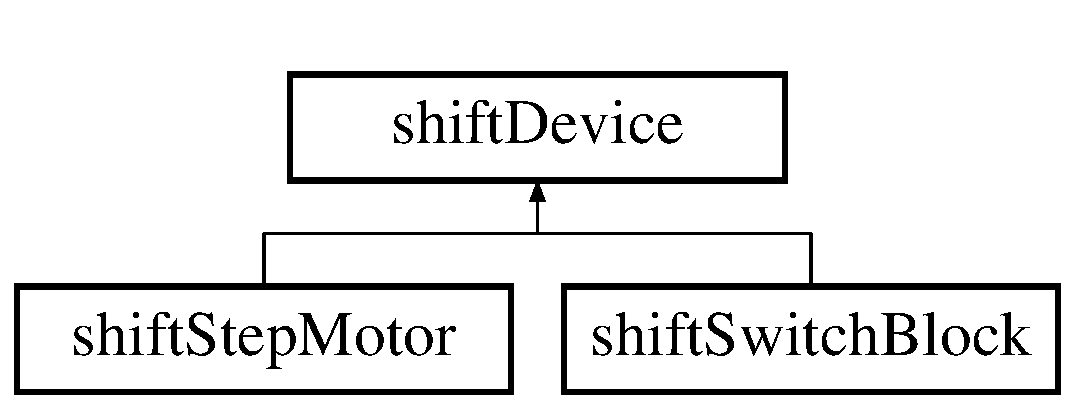
\includegraphics[height=2.000000cm]{classshift_device}
\end{center}
\end{figure}
\subsection*{Public Member Functions}
\begin{DoxyCompactItemize}
\item 
virtual void \hyperlink{classshift_device_ab67731aedf33aad1b8c6dcbdbd01ecff}{doDevTick} (uint8\_\-t bytesPerBoard, uint8\_\-t $\ast$boardBytes)
\begin{DoxyCompactList}\small\item\em Handle for the per timer tick behavior of each device. \item\end{DoxyCompactList}\item 
uint8\_\-t $\ast$ \hyperlink{classshift_device_a56b744e801a501975b323f4d3336b6f1}{getChannels} (void)
\begin{DoxyCompactList}\small\item\em Get the byte array that holds the channels that the device occupies. \item\end{DoxyCompactList}\item 
uint8\_\-t \hyperlink{classshift_device_a38f7799b9f1ae1269bba5da52fd84b4b}{getChanCount} (void)
\begin{DoxyCompactList}\small\item\em Get the number of channels the device occupies. \item\end{DoxyCompactList}\end{DoxyCompactItemize}
\subsection*{Protected Attributes}
\begin{DoxyCompactItemize}
\item 
uint8\_\-t $\ast$ \hyperlink{classshift_device_ac63a0543346c357134fd207a47976bab}{channels}
\begin{DoxyCompactList}\small\item\em Array of channels in the object relative to the board. \item\end{DoxyCompactList}\item 
uint8\_\-t \hyperlink{classshift_device_a8eed8391ef608036d0f55f42348c0e41}{chanCount}
\begin{DoxyCompactList}\small\item\em Number of channels per device, in device units. \item\end{DoxyCompactList}\end{DoxyCompactItemize}


\subsection{Detailed Description}
Abstract base class for creating devices such as motors that attach to a board. A \hyperlink{classshift_device}{shiftDevice} object represents an object controlled by a shift register board. 

\subsection{Member Function Documentation}
\hypertarget{classshift_device_ab67731aedf33aad1b8c6dcbdbd01ecff}{
\index{shiftDevice@{shiftDevice}!doDevTick@{doDevTick}}
\index{doDevTick@{doDevTick}!shiftDevice@{shiftDevice}}
\subsubsection[{doDevTick}]{\setlength{\rightskip}{0pt plus 5cm}virtual void shiftDevice::doDevTick (
\begin{DoxyParamCaption}
\item[{uint8\_\-t}]{ bytesPerBoard, }
\item[{uint8\_\-t $\ast$}]{ boardBytes}
\end{DoxyParamCaption}
)\hspace{0.3cm}{\ttfamily  \mbox{[}virtual\mbox{]}}}}
\label{classshift_device_ab67731aedf33aad1b8c6dcbdbd01ecff}


Handle for the per timer tick behavior of each device. 

This function is intended to be called from \hyperlink{classshift_board_a5a120f7aeb958c8e8fd0ec87eecc5798}{shiftBoard::doBoardTick()}, which passes it the array of bytes that it expects it to write the data to be shifted out to. 
\begin{DoxyParams}{Parameters}
{\em bytesPerBoard} & is the number of outgoing bytes for the board this device is part of. \\
\hline
{\em $\ast$boardBytes} & is the array of outgoing bytes for the board this device is part of.\\
\hline
\end{DoxyParams}
Must be re-\/implemented by each sub-\/class. 

Reimplemented in \hyperlink{classshift_step_motor_a9555644f6653ecaaf66611d26dd07959}{shiftStepMotor}, and \hyperlink{classshift_switch_block_ab6bbc5883fc7d966103df29d40ae012e}{shiftSwitchBlock}.

\hypertarget{classshift_device_a38f7799b9f1ae1269bba5da52fd84b4b}{
\index{shiftDevice@{shiftDevice}!getChanCount@{getChanCount}}
\index{getChanCount@{getChanCount}!shiftDevice@{shiftDevice}}
\subsubsection[{getChanCount}]{\setlength{\rightskip}{0pt plus 5cm}uint8\_\-t shiftDevice::getChanCount (
\begin{DoxyParamCaption}
\item[{void}]{}
\end{DoxyParamCaption}
)}}
\label{classshift_device_a38f7799b9f1ae1269bba5da52fd84b4b}


Get the number of channels the device occupies. 

\hypertarget{classshift_device_a56b744e801a501975b323f4d3336b6f1}{
\index{shiftDevice@{shiftDevice}!getChannels@{getChannels}}
\index{getChannels@{getChannels}!shiftDevice@{shiftDevice}}
\subsubsection[{getChannels}]{\setlength{\rightskip}{0pt plus 5cm}uint8\_\-t $\ast$ shiftDevice::getChannels (
\begin{DoxyParamCaption}
\item[{void}]{}
\end{DoxyParamCaption}
)}}
\label{classshift_device_a56b744e801a501975b323f4d3336b6f1}


Get the byte array that holds the channels that the device occupies. 



\subsection{Member Data Documentation}
\hypertarget{classshift_device_a8eed8391ef608036d0f55f42348c0e41}{
\index{shiftDevice@{shiftDevice}!chanCount@{chanCount}}
\index{chanCount@{chanCount}!shiftDevice@{shiftDevice}}
\subsubsection[{chanCount}]{\setlength{\rightskip}{0pt plus 5cm}uint8\_\-t {\bf shiftDevice::chanCount}\hspace{0.3cm}{\ttfamily  \mbox{[}protected\mbox{]}}}}
\label{classshift_device_a8eed8391ef608036d0f55f42348c0e41}


Number of channels per device, in device units. 

For example, a unipolar step motor consumes four switch channels. \hypertarget{classshift_device_ac63a0543346c357134fd207a47976bab}{
\index{shiftDevice@{shiftDevice}!channels@{channels}}
\index{channels@{channels}!shiftDevice@{shiftDevice}}
\subsubsection[{channels}]{\setlength{\rightskip}{0pt plus 5cm}uint8\_\-t$\ast$ {\bf shiftDevice::channels}\hspace{0.3cm}{\ttfamily  \mbox{[}protected\mbox{]}}}}
\label{classshift_device_ac63a0543346c357134fd207a47976bab}


Array of channels in the object relative to the board. 

This array holds the channel numbers. For example, a unipolar step motor might consume channel 1, 2, 3, and 4. This array would then be equal to \{1, 2, 3, 4\}. 

The documentation for this class was generated from the following files:\begin{DoxyCompactItemize}
\item 
C:/Users/Pierce/Desktop/arduino-\/0018/libraries/shiftStepper/\hyperlink{_shift_stepper_8h}{ShiftStepper.h}\item 
C:/Users/Pierce/Desktop/arduino-\/0018/libraries/shiftStepper/\hyperlink{_shift_stepper_8cpp}{ShiftStepper.cpp}\end{DoxyCompactItemize}

\hypertarget{classshift_six}{
\section{shiftSix Class Reference}
\label{classshift_six}\index{shiftSix@{shiftSix}}
}


Implementation of \hyperlink{classshift_board}{shiftBoard} for a six channel high current Arduino shield.  




{\ttfamily \#include $<$ShiftStepper.h$>$}

Inheritance diagram for shiftSix:\begin{figure}[H]
\begin{center}
\leavevmode
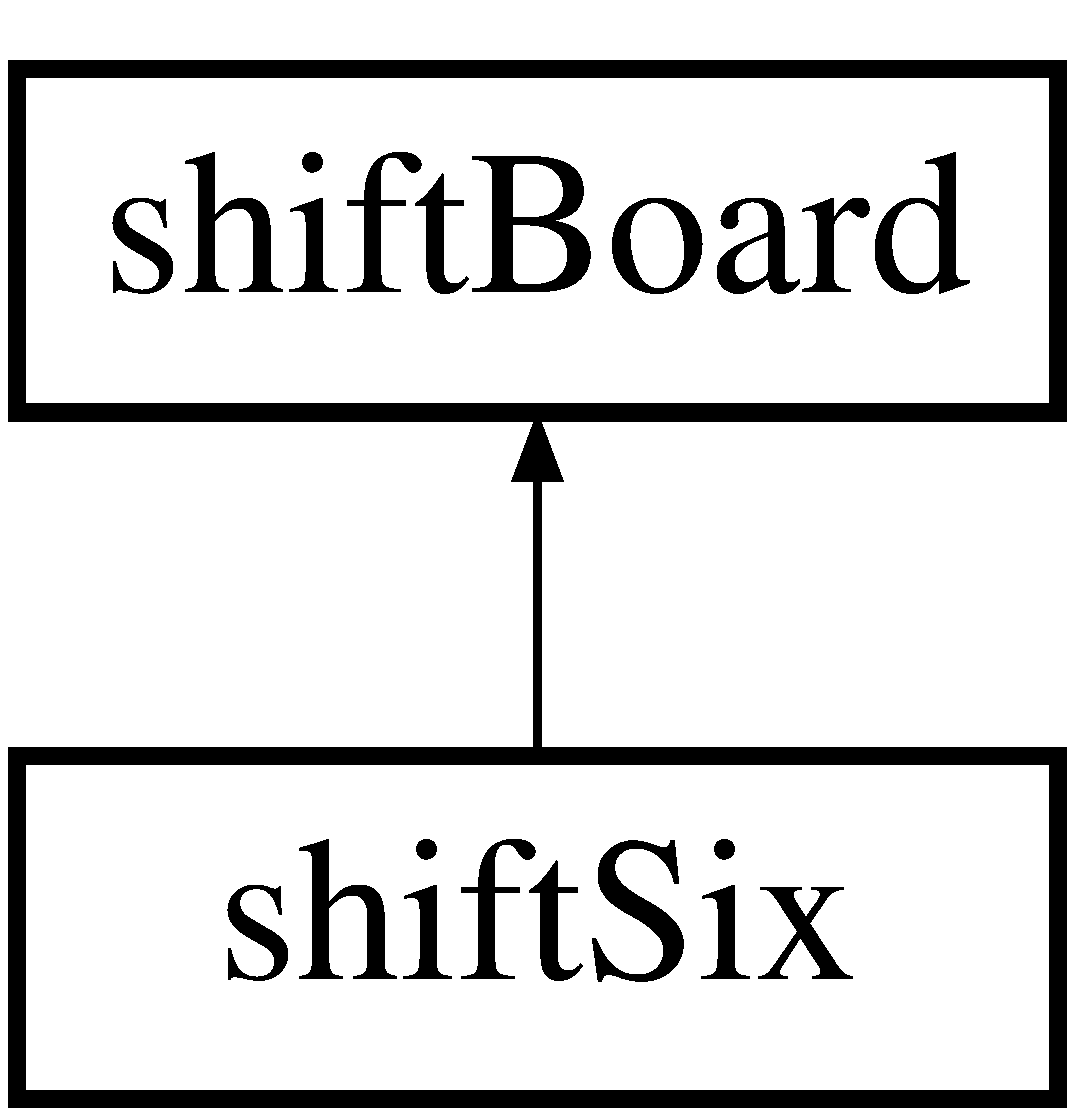
\includegraphics[height=2.000000cm]{classshift_six}
\end{center}
\end{figure}
\subsection*{Public Member Functions}
\begin{DoxyCompactItemize}
\item 
\hyperlink{classshift_six_a061ead17cbd393a561fa54146358c627}{shiftSix} (uint8\_\-t \hyperlink{classshift_board_ae7bba07850ced1219dcf67cab33de929}{devCount}, \hyperlink{classshift_device}{shiftDevice} $\ast$$\ast$\hyperlink{classshift_board_a07a2549714f7064fa5e48ec63fdb5efb}{devices})
\begin{DoxyCompactList}\small\item\em Create a new \hyperlink{classshift_six}{shiftSix} board object. \item\end{DoxyCompactList}\item 
void \hyperlink{classshift_six_aa69539cff7e19873a7d37e640632e966}{doBoardTick} (uint8\_\-t chainSize, uint8\_\-t firstByte, uint8\_\-t $\ast$chainBytes)
\begin{DoxyCompactList}\small\item\em Do a timer tick for a six channel board. \item\end{DoxyCompactList}\end{DoxyCompactItemize}


\subsection{Detailed Description}
Implementation of \hyperlink{classshift_board}{shiftBoard} for a six channel high current Arduino shield. 

\subsection{Constructor \& Destructor Documentation}
\hypertarget{classshift_six_a061ead17cbd393a561fa54146358c627}{
\index{shiftSix@{shiftSix}!shiftSix@{shiftSix}}
\index{shiftSix@{shiftSix}!shiftSix@{shiftSix}}
\subsubsection[{shiftSix}]{\setlength{\rightskip}{0pt plus 5cm}shiftSix::shiftSix (
\begin{DoxyParamCaption}
\item[{uint8\_\-t}]{ devCount, }
\item[{{\bf shiftDevice} $\ast$$\ast$}]{ devices}
\end{DoxyParamCaption}
)}}
\label{classshift_six_a061ead17cbd393a561fa54146358c627}


Create a new \hyperlink{classshift_six}{shiftSix} board object. 


\begin{DoxyParams}{Parameters}
{\em devCount} & The number of individual devices attached to this board. \\
\hline
{\em $\ast$$\ast$devices} & An array of pointers to the device objects. This array and the objects it contains must be allocated either statically or at global scope. \\
\hline
\end{DoxyParams}


\subsection{Member Function Documentation}
\hypertarget{classshift_six_aa69539cff7e19873a7d37e640632e966}{
\index{shiftSix@{shiftSix}!doBoardTick@{doBoardTick}}
\index{doBoardTick@{doBoardTick}!shiftSix@{shiftSix}}
\subsubsection[{doBoardTick}]{\setlength{\rightskip}{0pt plus 5cm}void shiftSix::doBoardTick (
\begin{DoxyParamCaption}
\item[{uint8\_\-t}]{ chainSize, }
\item[{uint8\_\-t}]{ firstByte, }
\item[{uint8\_\-t $\ast$}]{ chainBytes}
\end{DoxyParamCaption}
)\hspace{0.3cm}{\ttfamily  \mbox{[}virtual\mbox{]}}}}
\label{classshift_six_aa69539cff7e19873a7d37e640632e966}


Do a timer tick for a six channel board. 


\begin{DoxyParams}{Parameters}
{\em chainSize} & The number of bytes in the entire daisy chain of boards \\
\hline
{\em firstByte} & The index of the first byte assigned to this board \\
\hline
{\em $\ast$chainBytes} & The array of bytes that will be shifted out to the chain. \\
\hline
\end{DoxyParams}


Reimplemented from \hyperlink{classshift_board_a5a120f7aeb958c8e8fd0ec87eecc5798}{shiftBoard}.



The documentation for this class was generated from the following files:\begin{DoxyCompactItemize}
\item 
C:/Users/Pierce/Desktop/arduino-\/0018/libraries/shiftStepper/\hyperlink{_shift_stepper_8h}{ShiftStepper.h}\item 
C:/Users/Pierce/Desktop/arduino-\/0018/libraries/shiftStepper/\hyperlink{_shift_stepper_8cpp}{ShiftStepper.cpp}\end{DoxyCompactItemize}

\hypertarget{classshift_sixteen}{
\section{shiftSixteen Class Reference}
\label{classshift_sixteen}\index{shiftSixteen@{shiftSixteen}}
}


Implementation of \hyperlink{classshift_board}{shiftBoard} for a sixteen channel high current Arduino shield.  




{\ttfamily \#include $<$ShiftStepper.h$>$}

Inheritance diagram for shiftSixteen:\begin{figure}[H]
\begin{center}
\leavevmode
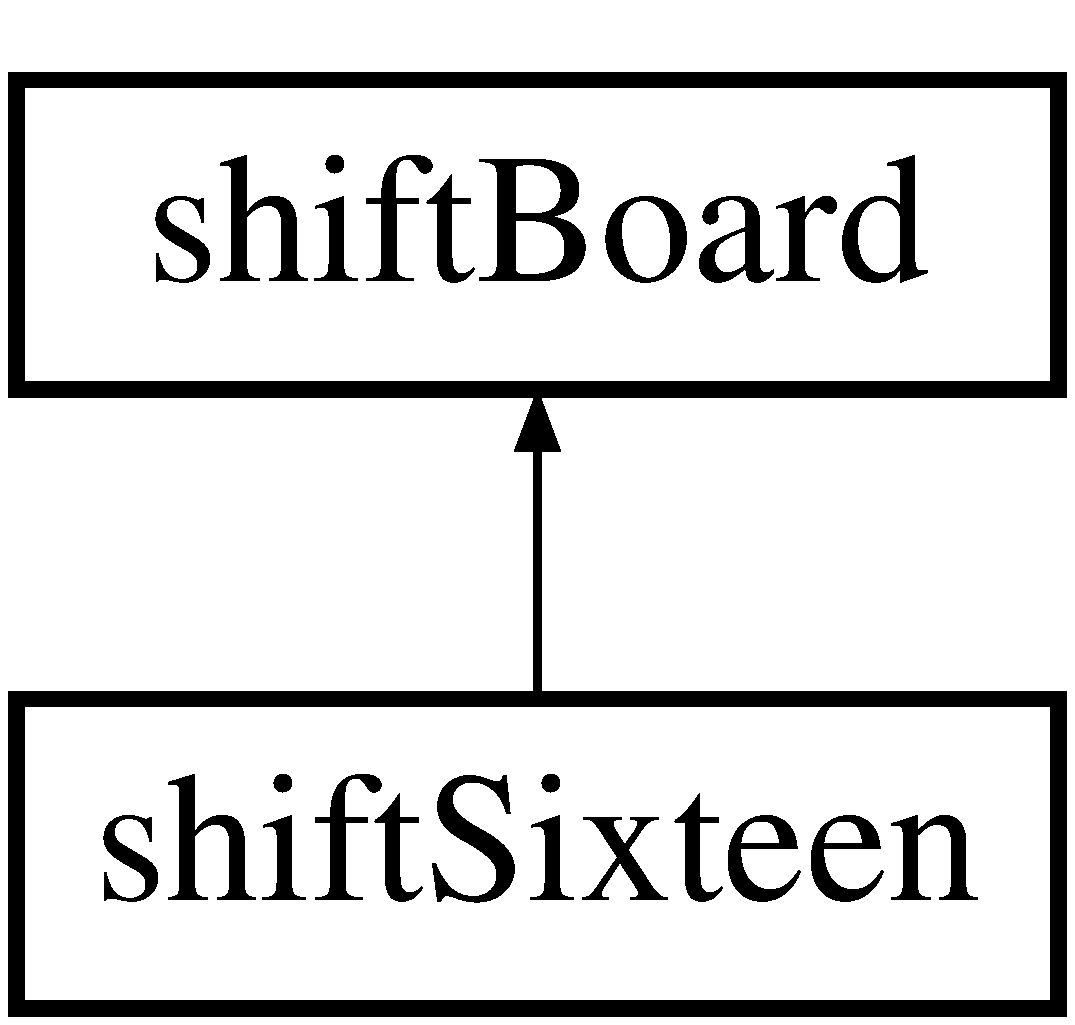
\includegraphics[height=2.000000cm]{classshift_sixteen}
\end{center}
\end{figure}
\subsection*{Public Member Functions}
\begin{DoxyCompactItemize}
\item 
\hyperlink{classshift_sixteen_afb8981ea1869387ca6e5b4c2a28b8018}{shiftSixteen} (uint8\_\-t \hyperlink{classshift_board_ae7bba07850ced1219dcf67cab33de929}{devCount}, \hyperlink{classshift_device}{shiftDevice} $\ast$$\ast$\hyperlink{classshift_board_a07a2549714f7064fa5e48ec63fdb5efb}{devices})
\begin{DoxyCompactList}\small\item\em Create a ShiftSixteen board object. \item\end{DoxyCompactList}\item 
void \hyperlink{classshift_sixteen_a28c2a73078d10abf6f779021fd8d2908}{doBoardTick} (uint8\_\-t chainSize, uint8\_\-t firstByte, uint8\_\-t $\ast$chainBytes)
\begin{DoxyCompactList}\small\item\em Do a timer tick for a sixteen channel board. \item\end{DoxyCompactList}\end{DoxyCompactItemize}


\subsection{Detailed Description}
Implementation of \hyperlink{classshift_board}{shiftBoard} for a sixteen channel high current Arduino shield. 

\subsection{Constructor \& Destructor Documentation}
\hypertarget{classshift_sixteen_afb8981ea1869387ca6e5b4c2a28b8018}{
\index{shiftSixteen@{shiftSixteen}!shiftSixteen@{shiftSixteen}}
\index{shiftSixteen@{shiftSixteen}!shiftSixteen@{shiftSixteen}}
\subsubsection[{shiftSixteen}]{\setlength{\rightskip}{0pt plus 5cm}shiftSixteen::shiftSixteen (
\begin{DoxyParamCaption}
\item[{uint8\_\-t}]{ devCount, }
\item[{{\bf shiftDevice} $\ast$$\ast$}]{ devices}
\end{DoxyParamCaption}
)}}
\label{classshift_sixteen_afb8981ea1869387ca6e5b4c2a28b8018}


Create a ShiftSixteen board object. 


\begin{DoxyParams}{Parameters}
{\em devCount} & The number of individual devices attached to this board. \\
\hline
{\em $\ast$$\ast$devices} & An array of pointers to the device objects. This array and the objects it contains must be allocated either statically or at global scope. \\
\hline
\end{DoxyParams}


\subsection{Member Function Documentation}
\hypertarget{classshift_sixteen_a28c2a73078d10abf6f779021fd8d2908}{
\index{shiftSixteen@{shiftSixteen}!doBoardTick@{doBoardTick}}
\index{doBoardTick@{doBoardTick}!shiftSixteen@{shiftSixteen}}
\subsubsection[{doBoardTick}]{\setlength{\rightskip}{0pt plus 5cm}void shiftSixteen::doBoardTick (
\begin{DoxyParamCaption}
\item[{uint8\_\-t}]{ chainSize, }
\item[{uint8\_\-t}]{ firstByte, }
\item[{uint8\_\-t $\ast$}]{ chainBytes}
\end{DoxyParamCaption}
)\hspace{0.3cm}{\ttfamily  \mbox{[}virtual\mbox{]}}}}
\label{classshift_sixteen_a28c2a73078d10abf6f779021fd8d2908}


Do a timer tick for a sixteen channel board. 


\begin{DoxyParams}{Parameters}
{\em chainSize} & The number of bytes in the entire daisy chain of boards \\
\hline
{\em firstByte} & The index of the first byte assigned to this board \\
\hline
{\em $\ast$chainBytes} & The array of bytes that will be shifted out to the chain. \\
\hline
\end{DoxyParams}


Reimplemented from \hyperlink{classshift_board_a5a120f7aeb958c8e8fd0ec87eecc5798}{shiftBoard}.



The documentation for this class was generated from the following files:\begin{DoxyCompactItemize}
\item 
C:/Users/Pierce/Desktop/arduino-\/0018/libraries/shiftStepper/\hyperlink{_shift_stepper_8h}{ShiftStepper.h}\item 
C:/Users/Pierce/Desktop/arduino-\/0018/libraries/shiftStepper/\hyperlink{_shift_stepper_8cpp}{ShiftStepper.cpp}\end{DoxyCompactItemize}

\hypertarget{classshift_step_motor}{
\section{shiftStepMotor Class Reference}
\label{classshift_step_motor}\index{shiftStepMotor@{shiftStepMotor}}
}


Implementation of a 4-\/phase unipolar stepper motor device.  




{\ttfamily \#include $<$ShiftStepper.h$>$}

Inheritance diagram for shiftStepMotor:\begin{figure}[H]
\begin{center}
\leavevmode
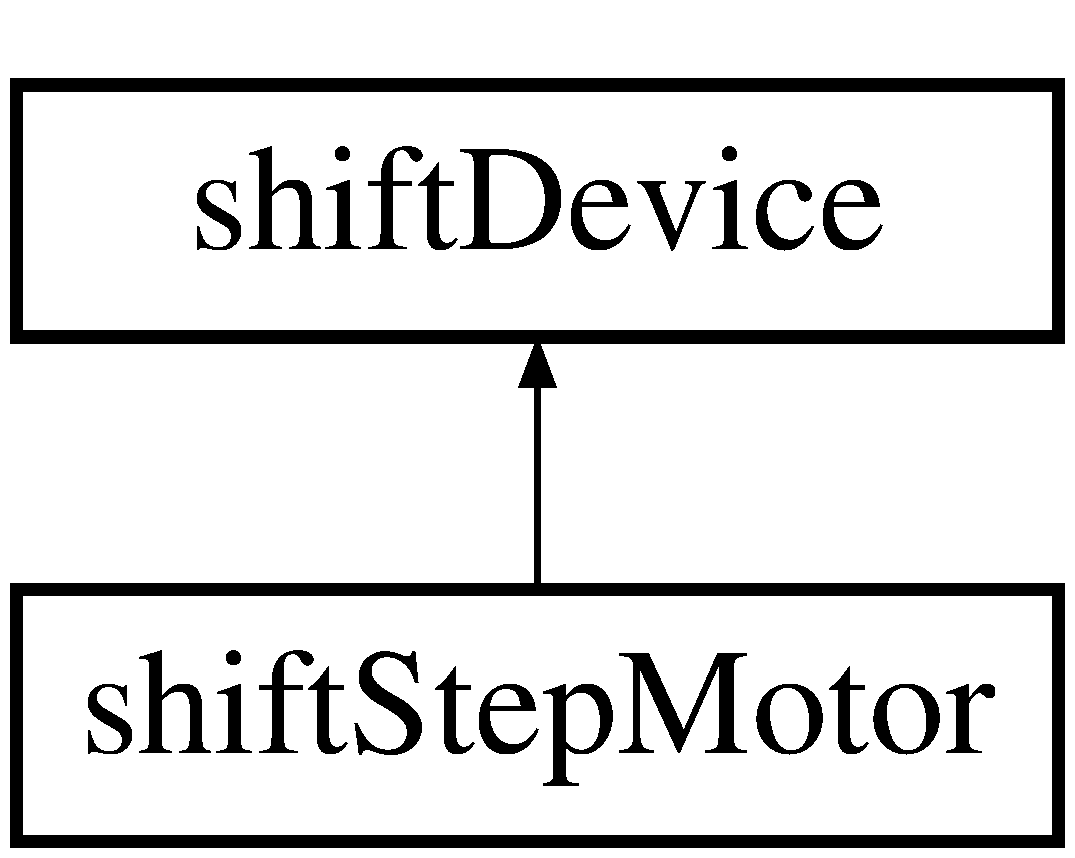
\includegraphics[height=2.000000cm]{classshift_step_motor}
\end{center}
\end{figure}
\subsection*{Public Member Functions}
\begin{DoxyCompactItemize}
\item 
\hyperlink{classshift_step_motor_aee8974e1496495ce45c7b43d0b42c464}{shiftStepMotor} (const uint8\_\-t seqSteps, const uint8\_\-t $\ast$sequence, const uint8\_\-t $\ast$channels)
\begin{DoxyCompactList}\small\item\em Creates a \hyperlink{classshift_step_motor}{shiftStepMotor} object. \item\end{DoxyCompactList}\item 
uint8\_\-t \hyperlink{classshift_step_motor_a463d9926c5bb4db38cea1a5d56c2c391}{incrStep} (int8\_\-t dir)
\begin{DoxyCompactList}\small\item\em Go one step in the commanded direction. \item\end{DoxyCompactList}\item 
uint8\_\-t \hyperlink{classshift_step_motor_aa93008b0f0485302d0512b85e9680df1}{doSteps} (int16\_\-t steps, int16\_\-t speed)
\begin{DoxyCompactList}\small\item\em Command a move of steps steps at speed speed. \item\end{DoxyCompactList}\item 
uint8\_\-t \hyperlink{classshift_step_motor_adc24feb4fba5e88460623f95f7c377e2}{setSpeed} (int16\_\-t speed)
\begin{DoxyCompactList}\small\item\em Set motor speed and direction. \item\end{DoxyCompactList}\item 
int16\_\-t \hyperlink{classshift_step_motor_a04f4a1dd0f970ea4937a3171ca965604}{getSpeed} (void)
\begin{DoxyCompactList}\small\item\em Get the current speed. \item\end{DoxyCompactList}\item 
int16\_\-t \hyperlink{classshift_step_motor_a1dcfe79646ef64dc6e97ff5488e68548}{getStepsToGo} (void)
\begin{DoxyCompactList}\small\item\em Get the number of steps to go in the current move. \item\end{DoxyCompactList}\item 
uint8\_\-t \hyperlink{classshift_step_motor_ae5f84d01eb0fd8226325aeb52ca401fb}{getSeqStep} (void)
\begin{DoxyCompactList}\small\item\em Returns the current output switch configuration. \item\end{DoxyCompactList}\item 
void \hyperlink{classshift_step_motor_a9555644f6653ecaaf66611d26dd07959}{doDevTick} (uint8\_\-t bytesPerBoard, uint8\_\-t $\ast$boardBytes)
\begin{DoxyCompactList}\small\item\em Local implementation of per timer tick behavior. \item\end{DoxyCompactList}\end{DoxyCompactItemize}


\subsection{Detailed Description}
Implementation of a 4-\/phase unipolar stepper motor device. 

\subsection{Constructor \& Destructor Documentation}
\hypertarget{classshift_step_motor_aee8974e1496495ce45c7b43d0b42c464}{
\index{shiftStepMotor@{shiftStepMotor}!shiftStepMotor@{shiftStepMotor}}
\index{shiftStepMotor@{shiftStepMotor}!shiftStepMotor@{shiftStepMotor}}
\subsubsection[{shiftStepMotor}]{\setlength{\rightskip}{0pt plus 5cm}shiftStepMotor::shiftStepMotor (
\begin{DoxyParamCaption}
\item[{const uint8\_\-t}]{ seqSteps, }
\item[{const uint8\_\-t $\ast$}]{ sequence, }
\item[{const uint8\_\-t $\ast$}]{ channels}
\end{DoxyParamCaption}
)}}
\label{classshift_step_motor_aee8974e1496495ce45c7b43d0b42c464}


Creates a \hyperlink{classshift_step_motor}{shiftStepMotor} object. 


\begin{DoxyParams}{Parameters}
{\em seqSteps} & The number of steps in the sequence of switch positions required to turn the motor. Typically 4 (full steps) or 8 (half steps). \\
\hline
{\em $\ast$sequence} & The array of switch positions for each step in the sequence. Bit 0 of each element of this array controls channels\mbox{[}0\mbox{]}, bit 1 controls channels\mbox{[}1\mbox{]}, etc. This array must have a number of elements equal to seqSteps. This array must be allocated either statically or at global scope. \\
\hline
{\em $\ast$channels} & The array of channel numbers used by the motor. Must have four elements. The order of the channels in this array determines how the members of sequence\mbox{[}\mbox{]} are interpreted. This array need not be permanently allocated. \\
\hline
\end{DoxyParams}


\subsection{Member Function Documentation}
\hypertarget{classshift_step_motor_a9555644f6653ecaaf66611d26dd07959}{
\index{shiftStepMotor@{shiftStepMotor}!doDevTick@{doDevTick}}
\index{doDevTick@{doDevTick}!shiftStepMotor@{shiftStepMotor}}
\subsubsection[{doDevTick}]{\setlength{\rightskip}{0pt plus 5cm}void shiftStepMotor::doDevTick (
\begin{DoxyParamCaption}
\item[{uint8\_\-t}]{ bytesPerBoard, }
\item[{uint8\_\-t $\ast$}]{ boardBytes}
\end{DoxyParamCaption}
)\hspace{0.3cm}{\ttfamily  \mbox{[}virtual\mbox{]}}}}
\label{classshift_step_motor_a9555644f6653ecaaf66611d26dd07959}


Local implementation of per timer tick behavior. 

This function manages the per-\/tick behavior of a stepper motor device. It is expected to be called from the doBoardTick() function of the board that contains this device.

It performs the following tasks:
\begin{DoxyItemize}
\item Checks whether or not it's time to make a step, based on the values of stepSpeed, lastStep, and stepsToGo
\item Writes the current switch state to the bits corresponding to the output channels in the boardBytes\mbox{[}\mbox{]} array
\end{DoxyItemize}


\begin{DoxyParams}{Parameters}
{\em bytesPerBoard} & This tells the function how many bytes of shift register are in the output board.\\
\hline
{\em $\ast$boardBytes} & This is a pointer to the array of bytes that the doBoardTick() function this is called from uses to write to the array of bytes that is then shifted out to the boards themselves. \\
\hline
\end{DoxyParams}


Reimplemented from \hyperlink{classshift_device_ab67731aedf33aad1b8c6dcbdbd01ecff}{shiftDevice}.

\hypertarget{classshift_step_motor_aa93008b0f0485302d0512b85e9680df1}{
\index{shiftStepMotor@{shiftStepMotor}!doSteps@{doSteps}}
\index{doSteps@{doSteps}!shiftStepMotor@{shiftStepMotor}}
\subsubsection[{doSteps}]{\setlength{\rightskip}{0pt plus 5cm}uint8\_\-t shiftStepMotor::doSteps (
\begin{DoxyParamCaption}
\item[{int16\_\-t}]{ steps, }
\item[{int16\_\-t}]{ speed}
\end{DoxyParamCaption}
)}}
\label{classshift_step_motor_aa93008b0f0485302d0512b85e9680df1}


Command a move of steps steps at speed speed. 


\begin{DoxyParams}{Parameters}
{\em steps} & The number of steps to move. If this number is negative, then this function commands continuous rotation. \\
\hline
{\em speed} & The speed at which to make the move. \\
\hline
\end{DoxyParams}
\begin{DoxyReturn}{Returns}
the error status. This feature has not been implemented, so it always returns 0 (success) 
\end{DoxyReturn}
\begin{DoxySeeAlso}{See also}
\hyperlink{classshift_step_motor_adc24feb4fba5e88460623f95f7c377e2}{shiftStepMotor::setSpeed()} for details on how the speed parameter works. 
\end{DoxySeeAlso}
\hypertarget{classshift_step_motor_ae5f84d01eb0fd8226325aeb52ca401fb}{
\index{shiftStepMotor@{shiftStepMotor}!getSeqStep@{getSeqStep}}
\index{getSeqStep@{getSeqStep}!shiftStepMotor@{shiftStepMotor}}
\subsubsection[{getSeqStep}]{\setlength{\rightskip}{0pt plus 5cm}uint8\_\-t shiftStepMotor::getSeqStep (
\begin{DoxyParamCaption}
\item[{void}]{}
\end{DoxyParamCaption}
)}}
\label{classshift_step_motor_ae5f84d01eb0fd8226325aeb52ca401fb}


Returns the current output switch configuration. 

\begin{DoxyReturn}{Returns}
a byte describing the state of the four switches that drive the stepper motor. 
\end{DoxyReturn}
\begin{DoxySeeAlso}{See also}
\hyperlink{classshift_step_motor_aee8974e1496495ce45c7b43d0b42c464}{shiftStepMotor::shiftStepMotor()} 
\end{DoxySeeAlso}
\hypertarget{classshift_step_motor_a04f4a1dd0f970ea4937a3171ca965604}{
\index{shiftStepMotor@{shiftStepMotor}!getSpeed@{getSpeed}}
\index{getSpeed@{getSpeed}!shiftStepMotor@{shiftStepMotor}}
\subsubsection[{getSpeed}]{\setlength{\rightskip}{0pt plus 5cm}int16\_\-t shiftStepMotor::getSpeed (
\begin{DoxyParamCaption}
\item[{void}]{}
\end{DoxyParamCaption}
)}}
\label{classshift_step_motor_a04f4a1dd0f970ea4937a3171ca965604}


Get the current speed. 

\begin{DoxyReturn}{Returns}
Speed value is in the same form as the input to \hyperlink{classshift_step_motor_adc24feb4fba5e88460623f95f7c377e2}{shiftStepMotor::setSpeed()}. It derives this from the internal representation by inverting the process described for that function. 
\end{DoxyReturn}
\begin{DoxySeeAlso}{See also}
\hyperlink{classshift_step_motor_adc24feb4fba5e88460623f95f7c377e2}{shiftStepMotor::setSpeed()} 
\end{DoxySeeAlso}
\hypertarget{classshift_step_motor_a1dcfe79646ef64dc6e97ff5488e68548}{
\index{shiftStepMotor@{shiftStepMotor}!getStepsToGo@{getStepsToGo}}
\index{getStepsToGo@{getStepsToGo}!shiftStepMotor@{shiftStepMotor}}
\subsubsection[{getStepsToGo}]{\setlength{\rightskip}{0pt plus 5cm}int16\_\-t shiftStepMotor::getStepsToGo (
\begin{DoxyParamCaption}
\item[{void}]{}
\end{DoxyParamCaption}
)}}
\label{classshift_step_motor_a1dcfe79646ef64dc6e97ff5488e68548}


Get the number of steps to go in the current move. 

\begin{DoxyReturn}{Returns}
The number of steps yet to go. A negative value commands continuous rotation. 
\end{DoxyReturn}
\begin{DoxySeeAlso}{See also}
\hyperlink{classshift_step_motor_aa93008b0f0485302d0512b85e9680df1}{shiftStepMotor::doSteps()}; 
\end{DoxySeeAlso}
\hypertarget{classshift_step_motor_a463d9926c5bb4db38cea1a5d56c2c391}{
\index{shiftStepMotor@{shiftStepMotor}!incrStep@{incrStep}}
\index{incrStep@{incrStep}!shiftStepMotor@{shiftStepMotor}}
\subsubsection[{incrStep}]{\setlength{\rightskip}{0pt plus 5cm}uint8\_\-t shiftStepMotor::incrStep (
\begin{DoxyParamCaption}
\item[{int8\_\-t}]{ dir}
\end{DoxyParamCaption}
)}}
\label{classshift_step_motor_a463d9926c5bb4db38cea1a5d56c2c391}


Go one step in the commanded direction. 

This function does one of three things, depending on the current state of the motor:
\begin{DoxyItemize}
\item If the motor is turning continuously (i.e. stepsToGo $<$ 0), it does nothing
\item If the motor is stopped (stepsToGo = 0), it does one step in the commanded direction
\item If the motor is in the middle of a commanded move, one step is added to the move in the commanded direction. If the move is positive and dir is positive, then one step will be added to the current move. If the move is positive and the dir is negative, one step will be subtracted for the current move.
\end{DoxyItemize}


\begin{DoxyParams}{Parameters}
{\em dir} & This defines the direction in which to perform the step. If dir $>$ 0, the step is positive; if dir $<$= 0, the step is negative. \\
\hline
\end{DoxyParams}
\begin{DoxyReturn}{Returns}
the error status. This feature has not been implemented, so it always returns 0 (success) 
\end{DoxyReturn}
\hypertarget{classshift_step_motor_adc24feb4fba5e88460623f95f7c377e2}{
\index{shiftStepMotor@{shiftStepMotor}!setSpeed@{setSpeed}}
\index{setSpeed@{setSpeed}!shiftStepMotor@{shiftStepMotor}}
\subsubsection[{setSpeed}]{\setlength{\rightskip}{0pt plus 5cm}uint8\_\-t shiftStepMotor::setSpeed (
\begin{DoxyParamCaption}
\item[{int16\_\-t}]{ speed}
\end{DoxyParamCaption}
)}}
\label{classshift_step_motor_adc24feb4fba5e88460623f95f7c377e2}


Set motor speed and direction. 

The most convenient way to represent the speed internally is as the number of \hyperlink{classshift_step_motor_a9555644f6653ecaaf66611d26dd07959}{doDevTick()} calls between steps. However, this is unwieldy to use, so this function simplifies it. \_\-\_\-maxMotorSpeed\_\-\_\- defines the maximum speed, and also the number of ticks that can be skipped per step. In order to determine the number of steps to skip, this function executes the following steps:
\begin{DoxyEnumerate}
\item Limit the speed parameter to between -\/\_\-\_\-maxMotorSpeed\_\-\_\- and \_\-\_\-maxMotorSpeed\_\-\_\-
\item If speed $>$ 0 (i.e. positive sense), set stepSpeed to \_\-\_\-maxMotorSpeed\_\-\_\- -\/ speed + 1
\item If speed $<$ 0 (i.e. negative sense), set stepSpeed to -\/\_\-\_\-maxMotorSpeed\_\-\_\- -\/ speed -\/ 1
\item If speed = 0 set stepSpeed to 0, i.e. no rotation
\end{DoxyEnumerate}


\begin{DoxyParams}{Parameters}
{\em speed} & The desired motor speed; sign indicates direction. \\
\hline
\end{DoxyParams}
\begin{DoxyReturn}{Returns}
the error status. This feature has not been implemented, so it always returns 0 (success) 
\end{DoxyReturn}


The documentation for this class was generated from the following files:\begin{DoxyCompactItemize}
\item 
C:/Users/Pierce/Desktop/arduino-\/0018/libraries/shiftStepper/\hyperlink{_shift_stepper_8h}{ShiftStepper.h}\item 
C:/Users/Pierce/Desktop/arduino-\/0018/libraries/shiftStepper/\hyperlink{_shift_stepper_8cpp}{ShiftStepper.cpp}\end{DoxyCompactItemize}

\hypertarget{classshift_switch_block}{
\section{shiftSwitchBlock Class Reference}
\label{classshift_switch_block}\index{shiftSwitchBlock@{shiftSwitchBlock}}
}


A block of plain switches.  




{\ttfamily \#include $<$ShiftStepper.h$>$}

Inheritance diagram for shiftSwitchBlock:\begin{figure}[H]
\begin{center}
\leavevmode
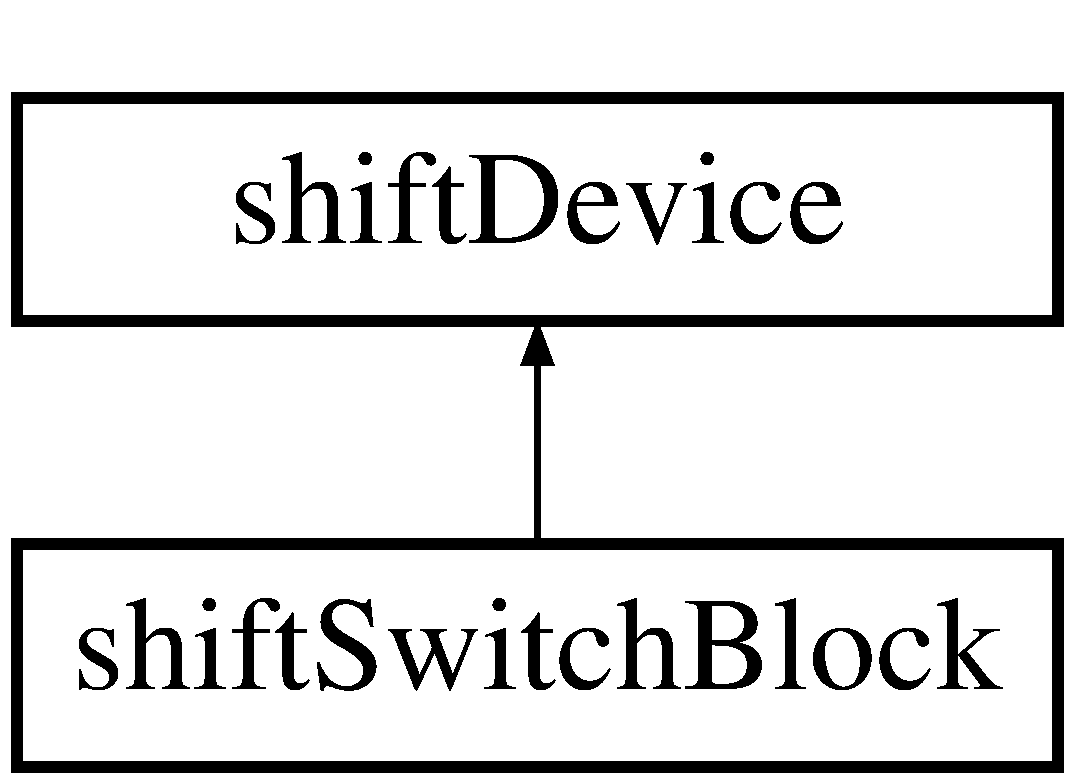
\includegraphics[height=2.000000cm]{classshift_switch_block}
\end{center}
\end{figure}
\subsection*{Public Member Functions}
\begin{DoxyCompactItemize}
\item 
\hyperlink{classshift_switch_block_a455f9d6bb935de28027746d01a14814c}{shiftStepMotor} (const uint8\_\-t $\ast$channels)
\item 
uint8\_\-t \hyperlink{classshift_switch_block_abc0f22095833ef9f9d84ae8b29934357}{setSwitches} (uint8\_\-t positions)
\begin{DoxyCompactList}\small\item\em Set switch positions. \item\end{DoxyCompactList}\item 
uint8\_\-t \hyperlink{classshift_switch_block_a292a158fc742c52f2227728c024e9e70}{getSwitches} (void)
\begin{DoxyCompactList}\small\item\em Get switch positions. \item\end{DoxyCompactList}\item 
void \hyperlink{classshift_switch_block_ab6bbc5883fc7d966103df29d40ae012e}{doDevTick} (uint8\_\-t bytesPerBoard, uint8\_\-t $\ast$boardBytes)
\begin{DoxyCompactList}\small\item\em Local implementation of per timer tick behavior. \item\end{DoxyCompactList}\end{DoxyCompactItemize}


\subsection{Detailed Description}
A block of plain switches. 

\subsection{Member Function Documentation}
\hypertarget{classshift_switch_block_ab6bbc5883fc7d966103df29d40ae012e}{
\index{shiftSwitchBlock@{shiftSwitchBlock}!doDevTick@{doDevTick}}
\index{doDevTick@{doDevTick}!shiftSwitchBlock@{shiftSwitchBlock}}
\subsubsection[{doDevTick}]{\setlength{\rightskip}{0pt plus 5cm}void shiftSwitchBlock::doDevTick (
\begin{DoxyParamCaption}
\item[{uint8\_\-t}]{ bytesPerBoard, }
\item[{uint8\_\-t $\ast$}]{ boardBytes}
\end{DoxyParamCaption}
)\hspace{0.3cm}{\ttfamily  \mbox{[}virtual\mbox{]}}}}
\label{classshift_switch_block_ab6bbc5883fc7d966103df29d40ae012e}


Local implementation of per timer tick behavior. 



Reimplemented from \hyperlink{classshift_device_ab67731aedf33aad1b8c6dcbdbd01ecff}{shiftDevice}.

\hypertarget{classshift_switch_block_a292a158fc742c52f2227728c024e9e70}{
\index{shiftSwitchBlock@{shiftSwitchBlock}!getSwitches@{getSwitches}}
\index{getSwitches@{getSwitches}!shiftSwitchBlock@{shiftSwitchBlock}}
\subsubsection[{getSwitches}]{\setlength{\rightskip}{0pt plus 5cm}uint8\_\-t shiftSwitchBlock::getSwitches (
\begin{DoxyParamCaption}
\item[{void}]{}
\end{DoxyParamCaption}
)}}
\label{classshift_switch_block_a292a158fc742c52f2227728c024e9e70}


Get switch positions. 

\hypertarget{classshift_switch_block_abc0f22095833ef9f9d84ae8b29934357}{
\index{shiftSwitchBlock@{shiftSwitchBlock}!setSwitches@{setSwitches}}
\index{setSwitches@{setSwitches}!shiftSwitchBlock@{shiftSwitchBlock}}
\subsubsection[{setSwitches}]{\setlength{\rightskip}{0pt plus 5cm}uint8\_\-t shiftSwitchBlock::setSwitches (
\begin{DoxyParamCaption}
\item[{uint8\_\-t}]{ positions}
\end{DoxyParamCaption}
)}}
\label{classshift_switch_block_abc0f22095833ef9f9d84ae8b29934357}


Set switch positions. 

\hypertarget{classshift_switch_block_a455f9d6bb935de28027746d01a14814c}{
\index{shiftSwitchBlock@{shiftSwitchBlock}!shiftStepMotor@{shiftStepMotor}}
\index{shiftStepMotor@{shiftStepMotor}!shiftSwitchBlock@{shiftSwitchBlock}}
\subsubsection[{shiftStepMotor}]{\setlength{\rightskip}{0pt plus 5cm}shiftSwitchBlock::shiftStepMotor (
\begin{DoxyParamCaption}
\item[{const uint8\_\-t $\ast$}]{ channels}
\end{DoxyParamCaption}
)}}
\label{classshift_switch_block_a455f9d6bb935de28027746d01a14814c}


The documentation for this class was generated from the following file:\begin{DoxyCompactItemize}
\item 
C:/Users/Pierce/Desktop/arduino-\/0018/libraries/shiftStepper/\hyperlink{_shift_stepper_8h}{ShiftStepper.h}\end{DoxyCompactItemize}

\chapter{File Documentation}
\hypertarget{_shift_stepper_8cpp}{
\section{C:/Users/Pierce/Desktop/arduino-\/0018/libraries/shiftStepper/ShiftStepper.cpp File Reference}
\label{_shift_stepper_8cpp}\index{C:/Users/Pierce/Desktop/arduino-\/0018/libraries/shiftStepper/ShiftStepper.cpp@{C:/Users/Pierce/Desktop/arduino-\/0018/libraries/shiftStepper/ShiftStepper.cpp}}
}
{\ttfamily \#include $<$stdio.h$>$}\par
{\ttfamily \#include $<$stdlib.h$>$}\par
{\ttfamily \#include $<$stdint.h$>$}\par
{\ttfamily \#include $<$avr/io.h$>$}\par
{\ttfamily \#include $<$inttypes.h$>$}\par
{\ttfamily \#include $<$avr/interrupt.h$>$}\par
{\ttfamily \#include \char`\"{}WProgram.h\char`\"{}}\par
{\ttfamily \#include \char`\"{}wiring.h\char`\"{}}\par
{\ttfamily \#include \char`\"{}wiring\_\-private.h\char`\"{}}\par
{\ttfamily \#include \char`\"{}pins\_\-arduino.h\char`\"{}}\par
{\ttfamily \#include \char`\"{}HardwareSerial.h\char`\"{}}\par
{\ttfamily \#include \char`\"{}shiftStepper.h\char`\"{}}\par
\subsection*{Defines}
\begin{DoxyCompactItemize}
\item 
\#define \hyperlink{_shift_stepper_8cpp_ae7701cd9aca25a5d2f3f9ac55dbc9f9f}{\_\-\_\-shiftSixteenBytes\_\-\_\-}~2
\item 
\#define \hyperlink{_shift_stepper_8cpp_a96af413ea9d141d8192568ae9425f363}{\_\-\_\-shiftSixteenFirst\_\-\_\-}~0
\item 
\#define \hyperlink{_shift_stepper_8cpp_ac5c0b389a81e12fc3319f49797c7024a}{\_\-\_\-shiftSixteenLast\_\-\_\-}~15
\item 
\#define \hyperlink{_shift_stepper_8cpp_aa603edb13f3837f481018aef04709dd5}{\_\-\_\-shiftSixBytes\_\-\_\-}~1
\item 
\#define \hyperlink{_shift_stepper_8cpp_a42e0c3a701a6b9c4e4564b150a9b2084}{\_\-\_\-shiftSixFirst\_\-\_\-}~1
\item 
\#define \hyperlink{_shift_stepper_8cpp_a386cb6b80acfa854979ebb8ff4e02c96}{\_\-\_\-shiftSixLast\_\-\_\-}~6
\end{DoxyCompactItemize}
\subsection*{Functions}
\begin{DoxyCompactItemize}
\item 
int \hyperlink{_shift_stepper_8cpp_ad9a42607fb7932f44ba914ac49972e62}{\_\-\_\-cxa\_\-guard\_\-acquire} (\_\-\_\-guard $\ast$g)
\item 
void \hyperlink{_shift_stepper_8cpp_adef76ddddaddf969efa3bfad968fd430}{\_\-\_\-cxa\_\-guard\_\-release} (\_\-\_\-guard $\ast$g)
\item 
void \hyperlink{_shift_stepper_8cpp_a357afb2dc20a652447f3a529dbda60e4}{\_\-\_\-cxa\_\-guard\_\-abort} (\_\-\_\-guard $\ast$)
\end{DoxyCompactItemize}


\subsection{Define Documentation}
\hypertarget{_shift_stepper_8cpp_aa603edb13f3837f481018aef04709dd5}{
\index{ShiftStepper.cpp@{ShiftStepper.cpp}!\_\-\_\-shiftSixBytes\_\-\_\-@{\_\-\_\-shiftSixBytes\_\-\_\-}}
\index{\_\-\_\-shiftSixBytes\_\-\_\-@{\_\-\_\-shiftSixBytes\_\-\_\-}!ShiftStepper.cpp@{ShiftStepper.cpp}}
\subsubsection[{\_\-\_\-shiftSixBytes\_\-\_\-}]{\setlength{\rightskip}{0pt plus 5cm}\#define \_\-\_\-shiftSixBytes\_\-\_\-~1}}
\label{_shift_stepper_8cpp_aa603edb13f3837f481018aef04709dd5}
\hypertarget{_shift_stepper_8cpp_a42e0c3a701a6b9c4e4564b150a9b2084}{
\index{ShiftStepper.cpp@{ShiftStepper.cpp}!\_\-\_\-shiftSixFirst\_\-\_\-@{\_\-\_\-shiftSixFirst\_\-\_\-}}
\index{\_\-\_\-shiftSixFirst\_\-\_\-@{\_\-\_\-shiftSixFirst\_\-\_\-}!ShiftStepper.cpp@{ShiftStepper.cpp}}
\subsubsection[{\_\-\_\-shiftSixFirst\_\-\_\-}]{\setlength{\rightskip}{0pt plus 5cm}\#define \_\-\_\-shiftSixFirst\_\-\_\-~1}}
\label{_shift_stepper_8cpp_a42e0c3a701a6b9c4e4564b150a9b2084}
\hypertarget{_shift_stepper_8cpp_a386cb6b80acfa854979ebb8ff4e02c96}{
\index{ShiftStepper.cpp@{ShiftStepper.cpp}!\_\-\_\-shiftSixLast\_\-\_\-@{\_\-\_\-shiftSixLast\_\-\_\-}}
\index{\_\-\_\-shiftSixLast\_\-\_\-@{\_\-\_\-shiftSixLast\_\-\_\-}!ShiftStepper.cpp@{ShiftStepper.cpp}}
\subsubsection[{\_\-\_\-shiftSixLast\_\-\_\-}]{\setlength{\rightskip}{0pt plus 5cm}\#define \_\-\_\-shiftSixLast\_\-\_\-~6}}
\label{_shift_stepper_8cpp_a386cb6b80acfa854979ebb8ff4e02c96}
\hypertarget{_shift_stepper_8cpp_ae7701cd9aca25a5d2f3f9ac55dbc9f9f}{
\index{ShiftStepper.cpp@{ShiftStepper.cpp}!\_\-\_\-shiftSixteenBytes\_\-\_\-@{\_\-\_\-shiftSixteenBytes\_\-\_\-}}
\index{\_\-\_\-shiftSixteenBytes\_\-\_\-@{\_\-\_\-shiftSixteenBytes\_\-\_\-}!ShiftStepper.cpp@{ShiftStepper.cpp}}
\subsubsection[{\_\-\_\-shiftSixteenBytes\_\-\_\-}]{\setlength{\rightskip}{0pt plus 5cm}\#define \_\-\_\-shiftSixteenBytes\_\-\_\-~2}}
\label{_shift_stepper_8cpp_ae7701cd9aca25a5d2f3f9ac55dbc9f9f}
\hypertarget{_shift_stepper_8cpp_a96af413ea9d141d8192568ae9425f363}{
\index{ShiftStepper.cpp@{ShiftStepper.cpp}!\_\-\_\-shiftSixteenFirst\_\-\_\-@{\_\-\_\-shiftSixteenFirst\_\-\_\-}}
\index{\_\-\_\-shiftSixteenFirst\_\-\_\-@{\_\-\_\-shiftSixteenFirst\_\-\_\-}!ShiftStepper.cpp@{ShiftStepper.cpp}}
\subsubsection[{\_\-\_\-shiftSixteenFirst\_\-\_\-}]{\setlength{\rightskip}{0pt plus 5cm}\#define \_\-\_\-shiftSixteenFirst\_\-\_\-~0}}
\label{_shift_stepper_8cpp_a96af413ea9d141d8192568ae9425f363}
\hypertarget{_shift_stepper_8cpp_ac5c0b389a81e12fc3319f49797c7024a}{
\index{ShiftStepper.cpp@{ShiftStepper.cpp}!\_\-\_\-shiftSixteenLast\_\-\_\-@{\_\-\_\-shiftSixteenLast\_\-\_\-}}
\index{\_\-\_\-shiftSixteenLast\_\-\_\-@{\_\-\_\-shiftSixteenLast\_\-\_\-}!ShiftStepper.cpp@{ShiftStepper.cpp}}
\subsubsection[{\_\-\_\-shiftSixteenLast\_\-\_\-}]{\setlength{\rightskip}{0pt plus 5cm}\#define \_\-\_\-shiftSixteenLast\_\-\_\-~15}}
\label{_shift_stepper_8cpp_ac5c0b389a81e12fc3319f49797c7024a}


\subsection{Function Documentation}
\hypertarget{_shift_stepper_8cpp_a357afb2dc20a652447f3a529dbda60e4}{
\index{ShiftStepper.cpp@{ShiftStepper.cpp}!\_\-\_\-cxa\_\-guard\_\-abort@{\_\-\_\-cxa\_\-guard\_\-abort}}
\index{\_\-\_\-cxa\_\-guard\_\-abort@{\_\-\_\-cxa\_\-guard\_\-abort}!ShiftStepper.cpp@{ShiftStepper.cpp}}
\subsubsection[{\_\-\_\-cxa\_\-guard\_\-abort}]{\setlength{\rightskip}{0pt plus 5cm}void \_\-\_\-cxa\_\-guard\_\-abort (
\begin{DoxyParamCaption}
\item[{\_\-\_\-guard $\ast$}]{}
\end{DoxyParamCaption}
)}}
\label{_shift_stepper_8cpp_a357afb2dc20a652447f3a529dbda60e4}
\hypertarget{_shift_stepper_8cpp_ad9a42607fb7932f44ba914ac49972e62}{
\index{ShiftStepper.cpp@{ShiftStepper.cpp}!\_\-\_\-cxa\_\-guard\_\-acquire@{\_\-\_\-cxa\_\-guard\_\-acquire}}
\index{\_\-\_\-cxa\_\-guard\_\-acquire@{\_\-\_\-cxa\_\-guard\_\-acquire}!ShiftStepper.cpp@{ShiftStepper.cpp}}
\subsubsection[{\_\-\_\-cxa\_\-guard\_\-acquire}]{\setlength{\rightskip}{0pt plus 5cm}int \_\-\_\-cxa\_\-guard\_\-acquire (
\begin{DoxyParamCaption}
\item[{\_\-\_\-guard $\ast$}]{ g}
\end{DoxyParamCaption}
)}}
\label{_shift_stepper_8cpp_ad9a42607fb7932f44ba914ac49972e62}
\hypertarget{_shift_stepper_8cpp_adef76ddddaddf969efa3bfad968fd430}{
\index{ShiftStepper.cpp@{ShiftStepper.cpp}!\_\-\_\-cxa\_\-guard\_\-release@{\_\-\_\-cxa\_\-guard\_\-release}}
\index{\_\-\_\-cxa\_\-guard\_\-release@{\_\-\_\-cxa\_\-guard\_\-release}!ShiftStepper.cpp@{ShiftStepper.cpp}}
\subsubsection[{\_\-\_\-cxa\_\-guard\_\-release}]{\setlength{\rightskip}{0pt plus 5cm}void \_\-\_\-cxa\_\-guard\_\-release (
\begin{DoxyParamCaption}
\item[{\_\-\_\-guard $\ast$}]{ g}
\end{DoxyParamCaption}
)}}
\label{_shift_stepper_8cpp_adef76ddddaddf969efa3bfad968fd430}

\hypertarget{_shift_stepper_8h}{
\section{C:/Users/Pierce/Desktop/arduino-\/0018/libraries/shiftStepper/ShiftStepper.h File Reference}
\label{_shift_stepper_8h}\index{C:/Users/Pierce/Desktop/arduino-\/0018/libraries/shiftStepper/ShiftStepper.h@{C:/Users/Pierce/Desktop/arduino-\/0018/libraries/shiftStepper/ShiftStepper.h}}
}
{\ttfamily \#include $<$stdint.h$>$}\par
{\ttfamily \#include $<$inttypes.h$>$}\par
{\ttfamily \#include $<$avr/io.h$>$}\par
\subsection*{Classes}
\begin{DoxyCompactItemize}
\item 
class \hyperlink{classshift_device}{shiftDevice}
\begin{DoxyCompactList}\small\item\em Abstract base class for creating devices such as motors that attach to a board. \item\end{DoxyCompactList}\item 
class \hyperlink{classshift_step_motor}{shiftStepMotor}
\begin{DoxyCompactList}\small\item\em Implementation of a 4-\/phase unipolar stepper motor device. \item\end{DoxyCompactList}\item 
class \hyperlink{classshift_switch_block}{shiftSwitchBlock}
\begin{DoxyCompactList}\small\item\em A block of plain switches. \item\end{DoxyCompactList}\item 
class \hyperlink{classshift_board}{shiftBoard}
\begin{DoxyCompactList}\small\item\em Abstract base class for individual boards with \hyperlink{classshift_device}{shiftDevice}. \item\end{DoxyCompactList}\item 
class \hyperlink{classshift_sixteen}{shiftSixteen}
\begin{DoxyCompactList}\small\item\em Implementation of \hyperlink{classshift_board}{shiftBoard} for a sixteen channel high current Arduino shield. \item\end{DoxyCompactList}\item 
class \hyperlink{classshift_six}{shiftSix}
\begin{DoxyCompactList}\small\item\em Implementation of \hyperlink{classshift_board}{shiftBoard} for a six channel high current Arduino shield. \item\end{DoxyCompactList}\item 
class \hyperlink{classshift_board_direct}{shiftBoardDirect}
\begin{DoxyCompactList}\small\item\em Abstract base class for individual boards, without \hyperlink{classshift_device}{shiftDevice} objects. \item\end{DoxyCompactList}\item 
class \hyperlink{classshift_sixteen_direct}{shiftSixteenDirect}
\begin{DoxyCompactList}\small\item\em Implementation of \hyperlink{classshift_board_direct}{shiftBoardDirect} for a sixteen channel high current Arduino shield. \item\end{DoxyCompactList}\item 
class \hyperlink{classshift_six_direct}{shiftSixDirect}
\begin{DoxyCompactList}\small\item\em Implementation of \hyperlink{classshift_board_direct}{shiftBoardDirect} for a six channel high current board. \item\end{DoxyCompactList}\item 
class \hyperlink{classshift_chain}{shiftChain}
\begin{DoxyCompactList}\small\item\em Class to represent a daisy chain of boards. \item\end{DoxyCompactList}\end{DoxyCompactItemize}
\subsection*{Defines}
\begin{DoxyCompactItemize}
\item 
\#define \hyperlink{_shift_stepper_8h_acd65c881d960ae17acb8c043d814d1ed}{\_\-\_\-channelsPerSwitchBlockDefault\_\-\_\-}~4
\begin{DoxyCompactList}\small\item\em Default number of channels in each \hyperlink{classshift_switch_block}{shiftSwitchBlock} device. \item\end{DoxyCompactList}\item 
\#define \hyperlink{_shift_stepper_8h_a0c275f5b5bbf9092eafd8f88f13efc63}{\_\-\_\-channelsPerSwitchBlockMax\_\-\_\-}~8
\begin{DoxyCompactList}\small\item\em Max number of channels in each \hyperlink{classshift_switch_block}{shiftSwitchBlock} device. \item\end{DoxyCompactList}\item 
\#define \hyperlink{_shift_stepper_8h_a19e74e78535a1c218485566fcc76751e}{\_\-\_\-channelsPerMotor\_\-\_\-}~4
\begin{DoxyCompactList}\small\item\em Number of channels each stepper motor consumes. \item\end{DoxyCompactList}\item 
\#define \hyperlink{_shift_stepper_8h_a2f33b141a2bcb279df22840ca9b96d5a}{\_\-\_\-maxMotorSpeed\_\-\_\-}~255
\begin{DoxyCompactList}\small\item\em Maximum speed of each motor. \item\end{DoxyCompactList}\item 
\#define \hyperlink{_shift_stepper_8h_a103bd7a2dfbff14ab2ff191f2fc170ea}{\_\-\_\-preScaler32\_\-\_\-}~3
\begin{DoxyCompactList}\small\item\em Sets timer pre-\/scaler to 32. \item\end{DoxyCompactList}\item 
\#define \hyperlink{_shift_stepper_8h_a67c5677f6507d03de981a1cd11ccc1c3}{\_\-\_\-preScaler64\_\-\_\-}~4
\begin{DoxyCompactList}\small\item\em Sets timer pre-\/scaler to 64. \item\end{DoxyCompactList}\item 
\#define \hyperlink{_shift_stepper_8h_aa8c20c8e76ea193c4d0ac4aa3aafe307}{\_\-\_\-preScaler128\_\-\_\-}~5
\begin{DoxyCompactList}\small\item\em Sets timer pre-\/scaler to 128. \item\end{DoxyCompactList}\item 
\#define \hyperlink{_shift_stepper_8h_a5934e1bfb2663597ce181f4f00c1b1c4}{\_\-\_\-preScaler256\_\-\_\-}~6
\begin{DoxyCompactList}\small\item\em Sets timer pre-\/scaler to 256. \item\end{DoxyCompactList}\item 
\#define \hyperlink{_shift_stepper_8h_a655d124c2726677785a75e0b24a4049a}{\_\-\_\-preScaler1024\_\-\_\-}~7
\begin{DoxyCompactList}\small\item\em Sets timer pre-\/scaler to 1024. \item\end{DoxyCompactList}\item 
\#define \hyperlink{_shift_stepper_8h_ae7701cd9aca25a5d2f3f9ac55dbc9f9f}{\_\-\_\-shiftSixteenBytes\_\-\_\-}~2
\begin{DoxyCompactList}\small\item\em The number of bytes on a sixteen channel board. \item\end{DoxyCompactList}\item 
\#define \hyperlink{_shift_stepper_8h_a96af413ea9d141d8192568ae9425f363}{\_\-\_\-shiftSixteenFirst\_\-\_\-}~0
\begin{DoxyCompactList}\small\item\em The index of the lowest channel on a six channel board. \item\end{DoxyCompactList}\item 
\#define \hyperlink{_shift_stepper_8h_ac5c0b389a81e12fc3319f49797c7024a}{\_\-\_\-shiftSixteenLast\_\-\_\-}~15
\begin{DoxyCompactList}\small\item\em The index of the highest channel on a six channel board. \item\end{DoxyCompactList}\item 
\#define \hyperlink{_shift_stepper_8h_aa603edb13f3837f481018aef04709dd5}{\_\-\_\-shiftSixBytes\_\-\_\-}~1
\begin{DoxyCompactList}\small\item\em The number of bytes on a six channel board. \item\end{DoxyCompactList}\item 
\#define \hyperlink{_shift_stepper_8h_a42e0c3a701a6b9c4e4564b150a9b2084}{\_\-\_\-shiftSixFirst\_\-\_\-}~1
\begin{DoxyCompactList}\small\item\em The index of the lowest channel on a six channel board. \item\end{DoxyCompactList}\item 
\#define \hyperlink{_shift_stepper_8h_a386cb6b80acfa854979ebb8ff4e02c96}{\_\-\_\-shiftSixLast\_\-\_\-}~6
\begin{DoxyCompactList}\small\item\em The index of the highest channel on a six channel board. \item\end{DoxyCompactList}\end{DoxyCompactItemize}
\subsection*{Functions}
\begin{DoxyCompactItemize}
\item 
\_\-\_\-extension\_\-\_\- typedef int \_\-\_\-guard \hyperlink{_shift_stepper_8h_aa5aa60072f4063655d5283b6d7b7ab44}{\_\-\_\-attribute\_\-\_\-} ((mode(\_\-\_\-DI\_\-\_\-)))
\item 
int \hyperlink{_shift_stepper_8h_a239ddd7f6e7ee1b05b59b2e56d8afb40}{\_\-\_\-cxa\_\-guard\_\-acquire} (\_\-\_\-guard $\ast$)
\item 
void \hyperlink{_shift_stepper_8h_aab72c37f0b3e6fc38d293bd4f8dd61ed}{\_\-\_\-cxa\_\-guard\_\-release} (\_\-\_\-guard $\ast$)
\item 
void \hyperlink{_shift_stepper_8h_a357afb2dc20a652447f3a529dbda60e4}{\_\-\_\-cxa\_\-guard\_\-abort} (\_\-\_\-guard $\ast$)
\end{DoxyCompactItemize}
\subsection*{Variables}
\begin{DoxyCompactItemize}
\item 
static const uint8\_\-t \hyperlink{_shift_stepper_8h_a59ec2655d4308a5b786a148e24aeeeb2}{default4StepSequence} \mbox{[}4\mbox{]} = \{0x1, 0x2, 0x4, 0x8\}
\begin{DoxyCompactList}\small\item\em Default step sequence for full stepping. \item\end{DoxyCompactList}\item 
static const uint8\_\-t \hyperlink{_shift_stepper_8h_a75822d85a113536a5092e7cdfbfef56e}{default8StepSequence} \mbox{[}8\mbox{]} = \{0x1,0x3,0x2,0x6,0x4,0xc,0x8,0x9\}
\begin{DoxyCompactList}\small\item\em Default step sequence for half stepping. \item\end{DoxyCompactList}\end{DoxyCompactItemize}


\subsection{Define Documentation}
\hypertarget{_shift_stepper_8h_a19e74e78535a1c218485566fcc76751e}{
\index{ShiftStepper.h@{ShiftStepper.h}!\_\-\_\-channelsPerMotor\_\-\_\-@{\_\-\_\-channelsPerMotor\_\-\_\-}}
\index{\_\-\_\-channelsPerMotor\_\-\_\-@{\_\-\_\-channelsPerMotor\_\-\_\-}!ShiftStepper.h@{ShiftStepper.h}}
\subsubsection[{\_\-\_\-channelsPerMotor\_\-\_\-}]{\setlength{\rightskip}{0pt plus 5cm}\#define \_\-\_\-channelsPerMotor\_\-\_\-~4}}
\label{_shift_stepper_8h_a19e74e78535a1c218485566fcc76751e}


Number of channels each stepper motor consumes. 

\hypertarget{_shift_stepper_8h_acd65c881d960ae17acb8c043d814d1ed}{
\index{ShiftStepper.h@{ShiftStepper.h}!\_\-\_\-channelsPerSwitchBlockDefault\_\-\_\-@{\_\-\_\-channelsPerSwitchBlockDefault\_\-\_\-}}
\index{\_\-\_\-channelsPerSwitchBlockDefault\_\-\_\-@{\_\-\_\-channelsPerSwitchBlockDefault\_\-\_\-}!ShiftStepper.h@{ShiftStepper.h}}
\subsubsection[{\_\-\_\-channelsPerSwitchBlockDefault\_\-\_\-}]{\setlength{\rightskip}{0pt plus 5cm}\#define \_\-\_\-channelsPerSwitchBlockDefault\_\-\_\-~4}}
\label{_shift_stepper_8h_acd65c881d960ae17acb8c043d814d1ed}


Default number of channels in each \hyperlink{classshift_switch_block}{shiftSwitchBlock} device. 

\hypertarget{_shift_stepper_8h_a0c275f5b5bbf9092eafd8f88f13efc63}{
\index{ShiftStepper.h@{ShiftStepper.h}!\_\-\_\-channelsPerSwitchBlockMax\_\-\_\-@{\_\-\_\-channelsPerSwitchBlockMax\_\-\_\-}}
\index{\_\-\_\-channelsPerSwitchBlockMax\_\-\_\-@{\_\-\_\-channelsPerSwitchBlockMax\_\-\_\-}!ShiftStepper.h@{ShiftStepper.h}}
\subsubsection[{\_\-\_\-channelsPerSwitchBlockMax\_\-\_\-}]{\setlength{\rightskip}{0pt plus 5cm}\#define \_\-\_\-channelsPerSwitchBlockMax\_\-\_\-~8}}
\label{_shift_stepper_8h_a0c275f5b5bbf9092eafd8f88f13efc63}


Max number of channels in each \hyperlink{classshift_switch_block}{shiftSwitchBlock} device. 

\hypertarget{_shift_stepper_8h_a2f33b141a2bcb279df22840ca9b96d5a}{
\index{ShiftStepper.h@{ShiftStepper.h}!\_\-\_\-maxMotorSpeed\_\-\_\-@{\_\-\_\-maxMotorSpeed\_\-\_\-}}
\index{\_\-\_\-maxMotorSpeed\_\-\_\-@{\_\-\_\-maxMotorSpeed\_\-\_\-}!ShiftStepper.h@{ShiftStepper.h}}
\subsubsection[{\_\-\_\-maxMotorSpeed\_\-\_\-}]{\setlength{\rightskip}{0pt plus 5cm}\#define \_\-\_\-maxMotorSpeed\_\-\_\-~255}}
\label{_shift_stepper_8h_a2f33b141a2bcb279df22840ca9b96d5a}


Maximum speed of each motor. 

\hypertarget{_shift_stepper_8h_a655d124c2726677785a75e0b24a4049a}{
\index{ShiftStepper.h@{ShiftStepper.h}!\_\-\_\-preScaler1024\_\-\_\-@{\_\-\_\-preScaler1024\_\-\_\-}}
\index{\_\-\_\-preScaler1024\_\-\_\-@{\_\-\_\-preScaler1024\_\-\_\-}!ShiftStepper.h@{ShiftStepper.h}}
\subsubsection[{\_\-\_\-preScaler1024\_\-\_\-}]{\setlength{\rightskip}{0pt plus 5cm}\#define \_\-\_\-preScaler1024\_\-\_\-~7}}
\label{_shift_stepper_8h_a655d124c2726677785a75e0b24a4049a}


Sets timer pre-\/scaler to 1024. 

\hypertarget{_shift_stepper_8h_aa8c20c8e76ea193c4d0ac4aa3aafe307}{
\index{ShiftStepper.h@{ShiftStepper.h}!\_\-\_\-preScaler128\_\-\_\-@{\_\-\_\-preScaler128\_\-\_\-}}
\index{\_\-\_\-preScaler128\_\-\_\-@{\_\-\_\-preScaler128\_\-\_\-}!ShiftStepper.h@{ShiftStepper.h}}
\subsubsection[{\_\-\_\-preScaler128\_\-\_\-}]{\setlength{\rightskip}{0pt plus 5cm}\#define \_\-\_\-preScaler128\_\-\_\-~5}}
\label{_shift_stepper_8h_aa8c20c8e76ea193c4d0ac4aa3aafe307}


Sets timer pre-\/scaler to 128. 

\hypertarget{_shift_stepper_8h_a5934e1bfb2663597ce181f4f00c1b1c4}{
\index{ShiftStepper.h@{ShiftStepper.h}!\_\-\_\-preScaler256\_\-\_\-@{\_\-\_\-preScaler256\_\-\_\-}}
\index{\_\-\_\-preScaler256\_\-\_\-@{\_\-\_\-preScaler256\_\-\_\-}!ShiftStepper.h@{ShiftStepper.h}}
\subsubsection[{\_\-\_\-preScaler256\_\-\_\-}]{\setlength{\rightskip}{0pt plus 5cm}\#define \_\-\_\-preScaler256\_\-\_\-~6}}
\label{_shift_stepper_8h_a5934e1bfb2663597ce181f4f00c1b1c4}


Sets timer pre-\/scaler to 256. 

\hypertarget{_shift_stepper_8h_a103bd7a2dfbff14ab2ff191f2fc170ea}{
\index{ShiftStepper.h@{ShiftStepper.h}!\_\-\_\-preScaler32\_\-\_\-@{\_\-\_\-preScaler32\_\-\_\-}}
\index{\_\-\_\-preScaler32\_\-\_\-@{\_\-\_\-preScaler32\_\-\_\-}!ShiftStepper.h@{ShiftStepper.h}}
\subsubsection[{\_\-\_\-preScaler32\_\-\_\-}]{\setlength{\rightskip}{0pt plus 5cm}\#define \_\-\_\-preScaler32\_\-\_\-~3}}
\label{_shift_stepper_8h_a103bd7a2dfbff14ab2ff191f2fc170ea}


Sets timer pre-\/scaler to 32. 

\hypertarget{_shift_stepper_8h_a67c5677f6507d03de981a1cd11ccc1c3}{
\index{ShiftStepper.h@{ShiftStepper.h}!\_\-\_\-preScaler64\_\-\_\-@{\_\-\_\-preScaler64\_\-\_\-}}
\index{\_\-\_\-preScaler64\_\-\_\-@{\_\-\_\-preScaler64\_\-\_\-}!ShiftStepper.h@{ShiftStepper.h}}
\subsubsection[{\_\-\_\-preScaler64\_\-\_\-}]{\setlength{\rightskip}{0pt plus 5cm}\#define \_\-\_\-preScaler64\_\-\_\-~4}}
\label{_shift_stepper_8h_a67c5677f6507d03de981a1cd11ccc1c3}


Sets timer pre-\/scaler to 64. 

\hypertarget{_shift_stepper_8h_aa603edb13f3837f481018aef04709dd5}{
\index{ShiftStepper.h@{ShiftStepper.h}!\_\-\_\-shiftSixBytes\_\-\_\-@{\_\-\_\-shiftSixBytes\_\-\_\-}}
\index{\_\-\_\-shiftSixBytes\_\-\_\-@{\_\-\_\-shiftSixBytes\_\-\_\-}!ShiftStepper.h@{ShiftStepper.h}}
\subsubsection[{\_\-\_\-shiftSixBytes\_\-\_\-}]{\setlength{\rightskip}{0pt plus 5cm}\#define \_\-\_\-shiftSixBytes\_\-\_\-~1}}
\label{_shift_stepper_8h_aa603edb13f3837f481018aef04709dd5}


The number of bytes on a six channel board. 

\hypertarget{_shift_stepper_8h_a42e0c3a701a6b9c4e4564b150a9b2084}{
\index{ShiftStepper.h@{ShiftStepper.h}!\_\-\_\-shiftSixFirst\_\-\_\-@{\_\-\_\-shiftSixFirst\_\-\_\-}}
\index{\_\-\_\-shiftSixFirst\_\-\_\-@{\_\-\_\-shiftSixFirst\_\-\_\-}!ShiftStepper.h@{ShiftStepper.h}}
\subsubsection[{\_\-\_\-shiftSixFirst\_\-\_\-}]{\setlength{\rightskip}{0pt plus 5cm}\#define \_\-\_\-shiftSixFirst\_\-\_\-~1}}
\label{_shift_stepper_8h_a42e0c3a701a6b9c4e4564b150a9b2084}


The index of the lowest channel on a six channel board. 

\hypertarget{_shift_stepper_8h_a386cb6b80acfa854979ebb8ff4e02c96}{
\index{ShiftStepper.h@{ShiftStepper.h}!\_\-\_\-shiftSixLast\_\-\_\-@{\_\-\_\-shiftSixLast\_\-\_\-}}
\index{\_\-\_\-shiftSixLast\_\-\_\-@{\_\-\_\-shiftSixLast\_\-\_\-}!ShiftStepper.h@{ShiftStepper.h}}
\subsubsection[{\_\-\_\-shiftSixLast\_\-\_\-}]{\setlength{\rightskip}{0pt plus 5cm}\#define \_\-\_\-shiftSixLast\_\-\_\-~6}}
\label{_shift_stepper_8h_a386cb6b80acfa854979ebb8ff4e02c96}


The index of the highest channel on a six channel board. 

\hypertarget{_shift_stepper_8h_ae7701cd9aca25a5d2f3f9ac55dbc9f9f}{
\index{ShiftStepper.h@{ShiftStepper.h}!\_\-\_\-shiftSixteenBytes\_\-\_\-@{\_\-\_\-shiftSixteenBytes\_\-\_\-}}
\index{\_\-\_\-shiftSixteenBytes\_\-\_\-@{\_\-\_\-shiftSixteenBytes\_\-\_\-}!ShiftStepper.h@{ShiftStepper.h}}
\subsubsection[{\_\-\_\-shiftSixteenBytes\_\-\_\-}]{\setlength{\rightskip}{0pt plus 5cm}\#define \_\-\_\-shiftSixteenBytes\_\-\_\-~2}}
\label{_shift_stepper_8h_ae7701cd9aca25a5d2f3f9ac55dbc9f9f}


The number of bytes on a sixteen channel board. 

\hypertarget{_shift_stepper_8h_a96af413ea9d141d8192568ae9425f363}{
\index{ShiftStepper.h@{ShiftStepper.h}!\_\-\_\-shiftSixteenFirst\_\-\_\-@{\_\-\_\-shiftSixteenFirst\_\-\_\-}}
\index{\_\-\_\-shiftSixteenFirst\_\-\_\-@{\_\-\_\-shiftSixteenFirst\_\-\_\-}!ShiftStepper.h@{ShiftStepper.h}}
\subsubsection[{\_\-\_\-shiftSixteenFirst\_\-\_\-}]{\setlength{\rightskip}{0pt plus 5cm}\#define \_\-\_\-shiftSixteenFirst\_\-\_\-~0}}
\label{_shift_stepper_8h_a96af413ea9d141d8192568ae9425f363}


The index of the lowest channel on a six channel board. 

\hypertarget{_shift_stepper_8h_ac5c0b389a81e12fc3319f49797c7024a}{
\index{ShiftStepper.h@{ShiftStepper.h}!\_\-\_\-shiftSixteenLast\_\-\_\-@{\_\-\_\-shiftSixteenLast\_\-\_\-}}
\index{\_\-\_\-shiftSixteenLast\_\-\_\-@{\_\-\_\-shiftSixteenLast\_\-\_\-}!ShiftStepper.h@{ShiftStepper.h}}
\subsubsection[{\_\-\_\-shiftSixteenLast\_\-\_\-}]{\setlength{\rightskip}{0pt plus 5cm}\#define \_\-\_\-shiftSixteenLast\_\-\_\-~15}}
\label{_shift_stepper_8h_ac5c0b389a81e12fc3319f49797c7024a}


The index of the highest channel on a six channel board. 



\subsection{Function Documentation}
\hypertarget{_shift_stepper_8h_aa5aa60072f4063655d5283b6d7b7ab44}{
\index{ShiftStepper.h@{ShiftStepper.h}!\_\-\_\-attribute\_\-\_\-@{\_\-\_\-attribute\_\-\_\-}}
\index{\_\-\_\-attribute\_\-\_\-@{\_\-\_\-attribute\_\-\_\-}!ShiftStepper.h@{ShiftStepper.h}}
\subsubsection[{\_\-\_\-attribute\_\-\_\-}]{\setlength{\rightskip}{0pt plus 5cm}\_\-\_\-extension\_\-\_\- typedef int \_\-\_\-guard \_\-\_\-attribute\_\-\_\- (
\begin{DoxyParamCaption}
\item[{(mode(\_\-\_\-DI\_\-\_\-))}]{}
\end{DoxyParamCaption}
)}}
\label{_shift_stepper_8h_aa5aa60072f4063655d5283b6d7b7ab44}
This is some strange linker food required to make it all work.

See \href{http://www.avrfreaks.net/index.php?name=PNphpBB2&file=viewtopic&p=410870}{\tt http://www.avrfreaks.net/index.php?name=PNphpBB2\&file=viewtopic\&p=410870} \hypertarget{_shift_stepper_8h_a357afb2dc20a652447f3a529dbda60e4}{
\index{ShiftStepper.h@{ShiftStepper.h}!\_\-\_\-cxa\_\-guard\_\-abort@{\_\-\_\-cxa\_\-guard\_\-abort}}
\index{\_\-\_\-cxa\_\-guard\_\-abort@{\_\-\_\-cxa\_\-guard\_\-abort}!ShiftStepper.h@{ShiftStepper.h}}
\subsubsection[{\_\-\_\-cxa\_\-guard\_\-abort}]{\setlength{\rightskip}{0pt plus 5cm}void \_\-\_\-cxa\_\-guard\_\-abort (
\begin{DoxyParamCaption}
\item[{\_\-\_\-guard $\ast$}]{}
\end{DoxyParamCaption}
)}}
\label{_shift_stepper_8h_a357afb2dc20a652447f3a529dbda60e4}
This is some strange linker food required to make it all work.

See \href{http://www.avrfreaks.net/index.php?name=PNphpBB2&file=viewtopic&p=410870}{\tt http://www.avrfreaks.net/index.php?name=PNphpBB2\&file=viewtopic\&p=410870} \hypertarget{_shift_stepper_8h_a239ddd7f6e7ee1b05b59b2e56d8afb40}{
\index{ShiftStepper.h@{ShiftStepper.h}!\_\-\_\-cxa\_\-guard\_\-acquire@{\_\-\_\-cxa\_\-guard\_\-acquire}}
\index{\_\-\_\-cxa\_\-guard\_\-acquire@{\_\-\_\-cxa\_\-guard\_\-acquire}!ShiftStepper.h@{ShiftStepper.h}}
\subsubsection[{\_\-\_\-cxa\_\-guard\_\-acquire}]{\setlength{\rightskip}{0pt plus 5cm}int \_\-\_\-cxa\_\-guard\_\-acquire (
\begin{DoxyParamCaption}
\item[{\_\-\_\-guard $\ast$}]{ g}
\end{DoxyParamCaption}
)}}
\label{_shift_stepper_8h_a239ddd7f6e7ee1b05b59b2e56d8afb40}
This is some strange linker food required to make it all work.

See \href{http://www.avrfreaks.net/index.php?name=PNphpBB2&file=viewtopic&p=410870}{\tt http://www.avrfreaks.net/index.php?name=PNphpBB2\&file=viewtopic\&p=410870} \hypertarget{_shift_stepper_8h_aab72c37f0b3e6fc38d293bd4f8dd61ed}{
\index{ShiftStepper.h@{ShiftStepper.h}!\_\-\_\-cxa\_\-guard\_\-release@{\_\-\_\-cxa\_\-guard\_\-release}}
\index{\_\-\_\-cxa\_\-guard\_\-release@{\_\-\_\-cxa\_\-guard\_\-release}!ShiftStepper.h@{ShiftStepper.h}}
\subsubsection[{\_\-\_\-cxa\_\-guard\_\-release}]{\setlength{\rightskip}{0pt plus 5cm}void \_\-\_\-cxa\_\-guard\_\-release (
\begin{DoxyParamCaption}
\item[{\_\-\_\-guard $\ast$}]{ g}
\end{DoxyParamCaption}
)}}
\label{_shift_stepper_8h_aab72c37f0b3e6fc38d293bd4f8dd61ed}
This is some strange linker food required to make it all work.

See \href{http://www.avrfreaks.net/index.php?name=PNphpBB2&file=viewtopic&p=410870}{\tt http://www.avrfreaks.net/index.php?name=PNphpBB2\&file=viewtopic\&p=410870} 

\subsection{Variable Documentation}
\hypertarget{_shift_stepper_8h_a59ec2655d4308a5b786a148e24aeeeb2}{
\index{ShiftStepper.h@{ShiftStepper.h}!default4StepSequence@{default4StepSequence}}
\index{default4StepSequence@{default4StepSequence}!ShiftStepper.h@{ShiftStepper.h}}
\subsubsection[{default4StepSequence}]{\setlength{\rightskip}{0pt plus 5cm}const uint8\_\-t {\bf default4StepSequence}\mbox{[}4\mbox{]} = \{0x1, 0x2, 0x4, 0x8\}\hspace{0.3cm}{\ttfamily  \mbox{[}static\mbox{]}}}}
\label{_shift_stepper_8h_a59ec2655d4308a5b786a148e24aeeeb2}


Default step sequence for full stepping. 

See \href{http://www.cs.uiowa.edu/~jones/step/types.html#unipolar}{\tt http://www.cs.uiowa.edu/$\sim$jones/step/types.html\#unipolar} for more details \hypertarget{_shift_stepper_8h_a75822d85a113536a5092e7cdfbfef56e}{
\index{ShiftStepper.h@{ShiftStepper.h}!default8StepSequence@{default8StepSequence}}
\index{default8StepSequence@{default8StepSequence}!ShiftStepper.h@{ShiftStepper.h}}
\subsubsection[{default8StepSequence}]{\setlength{\rightskip}{0pt plus 5cm}const uint8\_\-t {\bf default8StepSequence}\mbox{[}8\mbox{]} = \{0x1,0x3,0x2,0x6,0x4,0xc,0x8,0x9\}\hspace{0.3cm}{\ttfamily  \mbox{[}static\mbox{]}}}}
\label{_shift_stepper_8h_a75822d85a113536a5092e7cdfbfef56e}


Default step sequence for half stepping. 

See \href{http://www.cs.uiowa.edu/~jones/step/types.html#unipolar}{\tt http://www.cs.uiowa.edu/$\sim$jones/step/types.html\#unipolar} for more details 
\printindex
\end{document}
